% Some general notes:
%
% - keep lines short, to improve the merge of versions

\documentclass[11pt,a4paper,twoside]{article}
\usepackage{tascar}
\usepackage{amsmath}
\usepackage[utf8]{inputenc}
\usepackage{caption}
\usepackage{subcaption}
\DeclareMathOperator*{\argmax}{arg\,max}
\DeclareMathOperator*{\argmin}{arg\,min}
\usepackage{mathtools}
\usepackage{listings}
\usepackage{framed,color}
\usepackage{tabularx}
\definecolor{shadecolor}{rgb}{1,0.9,0.8}

\definecolor{mygreen}{rgb}{0,0.6,0}
\definecolor{mygray}{rgb}{0.5,0.5,0.5}
\definecolor{mygraybg}{rgb}{0.9,0.95,0.95}
\definecolor{mymauve}{rgb}{0.58,0,0.82}
\definecolor{bole}{rgb}{0.47, 0.27, 0.23}

\newenvironment{tscattributes}
{\begin{snugshade}
\begin{tabular}{p{0.25\columnwidth}p{0.7\columnwidth}}
{\bf Attributes:}\\
\hline
}{
\hline
\end{tabular}
\end{snugshade}
}

%\newenvironment{tscattr}[1]{
%  %\begin{snugshade}
%    \begin{tabularx}{\textwidth}{lllX}
%      \multicolumn{4}{l}{Element {\bf #1}}\\
%      \hline
%}{
%  \hline
%    \end{tabularx}
%  %\end{snugshade}
%}

\newenvironment{tscelements}
{\begin{snugshade}
\begin{tabular}{p{0.97\columnwidth}}
{\bf Sub-elements:}\\
\hline
}{
\\\hline
\end{tabular}
\end{snugshade}
}



\DeclarePairedDelimiterX{\norm}[1]{\lVert}{\rVert}{#1}

\begin{document}
\MHAtitle{User Manual}

TASCAR version \input{version.tex} (\today)
\fancyfoot[LE]{\fancyplain{}{\input{version.tex}}}
\fancyfoot[RO]{\fancyplain{}{\input{version.tex}}}

\newpage
\tableofcontents
\newpage
\pagenumbering{arabic}

\renewcommand{\ttdefault}{pcr}

\newtcbox{\attrbox}{nobeforeafter,tcbox raise base,
arc=0pt,outer arc=0pt,colback=mygraybg,colframe=black,
boxsep=0pt,left=1pt,right=1pt,top=2pt,bottom=2pt,
boxrule=0.2pt,fontupper=\small\ttfamily}

\newtcbox{\keybbox}{nobeforeafter,tcbox raise base,
arc=2pt,outer arc=2pt,colback=mygraybg,colframe=black,
boxsep=0pt,left=1pt,right=1pt,top=2pt,bottom=2pt,
boxrule=0.2pt,fontupper=\small\ttfamily}

\newtcbox{\elembox}{nobeforeafter,tcbox raise base,
arc=0pt,outer arc=0pt,colback=mygraybg,colframe=black,colupper=h4aBlueDark,
boxsep=0pt,left=1pt,right=1pt,top=2pt,bottom=2pt,
boxrule=0.2pt,fontupper=\small\ttfamily\bfseries}

\newcommand{\refelem}[2][]{
  \ifthenelse{\equal{#1}{}}{
    \hyperref[sec:#2]{\elembox{<#2/>}}
  }{
    \hyperref[sec:#1]{\elembox{<#2/>}}
  }
  %\index{#2}
}
\newcommand{\elem}[1]{\elembox{<#1/>}\index{#1 (XML element)}}
\newcommand{\indattr}[1]{\attrbox{\lstinline{#1}}\index{#1 (XML attribute)}}
\newcommand{\attr}[1]{\attrbox{\lstinline{#1}}}
\newcommand{\indmod}[1]{\hyperref[sec:#1]{{\bf #1}}\index{#1 (module)}}
\newcommand{\indapmod}[2][]{
  \ifthenelse{\equal{#1}{}}{
    \hyperref[sec:ap_#2]{{\bf #2}}\index{#2 (audio plugin)}
  }{
    \hyperref[sec:ap_#1]{{\bf #2}}\index{#2 (audio plugin)}
  }
}
\newcommand{\indrecgen}[2][]{
  \ifthenelse{\equal{#1}{}}{
    \hyperref[sec:recgen_#2]{{\bf #2}}
  }{
    \hyperref[sec:recgen_#1]{{\bf #2}}
  }
}
\newcommand{\indrecspk}[2][]{
  \ifthenelse{\equal{#1}{}}{
    \hyperref[sec:recspk_#2]{{\bf #2}}
  }{
    \hyperref[sec:recspk_#1]{{\bf #2}}
  }
}
\newcommand{\indrecrev}[2][]{
  \ifthenelse{\equal{#1}{}}{
    \hyperref[sec:recrev_#2]{{\bf #2}}
  }{
    \hyperref[sec:recrev_#1]{{\bf #2}}
  }
}
\newcommand{\keyb}[1]{\keybbox{\lstinline{#1}}}

\section*{Preface}

This user manual is -- as the whole \tascar{} toolbox -- work in
progress. Bug reports and feature wishes, like, for example, improved
documentation of specific features, should directly sent to any of the
authors of \tascar{}.

\section{Introduction}

\tascar{} -- toolbox for acoustic scene creation and rendering -- is a
software designed for rendering virtual acoustic environments
\citep{Grimm2015a,Grimm2016a,Grimm2019}.
%
In \tascar{} we can design virtual acoustic environments, which we
call acoustic {\em scenes} here, which are then rendered in real time
and can be played back using an arbitrary playback system.
%
These virtual acoustic scenes made using \tascar{} can also be
interactively explored by the user in the real time for example using
headphones and a joy-stick to steer the movement in acoustic space.
%
Direct sound paths as well as image sources generated by a geometric
image source model can be dynamically rendered.
%
However, it should be noted, that \tascar{} is not a room acoustics
simulator and the goal of \tascar{} is not to exactly reproduce the
sound field in a room, but to provide a fast and perceptively
plausible method for rendering virtual acoustic environments in real
time.
%
The \tascar{} software is suited for building dynamic and interactive
environments, which can be applied in hearing aid development and
evaluation, psycho-physics with adaptive changes of the spatial
configuration, soundscape simulations and computer games.
%
%There is almost unlimited variety of the environments, which can be
%simulated using \tascar{} and a user has an opportunity to specify the
%content and dynamics of an acoustic scene very precisely.

An acoustic scene in its simplest form consists of three types of
objects: sound sources, receiver and reflectors.
%
Each object has a position and orientation in the virtual space in a
given time.
%
To simulate an object in motion, the object's position or orientation
have to change over time.

The position of the receiver corresponds to the point in the virtual
space for which the simulation is rendered, while the receiver's
orientation influences the received sound, based on effective relative
direction of arrival, if the used receiver type is not
omni-directional.
%
To simulate the sound field at the receiver's position, some acoustic
phenomena like reflections, air absorption or diffraction are
mimicked.
%
These acoustic simulation methods will be discussed in detail in the
second chapter.

A list of \tascar{}-rendered scenes is described in \citet{Grimm2016}
and \citet{Hendrikse2019a}.
%
Validation of the principle applicability to hearing aid research can
be found in \citet{Grimm2015b}.
%
Distance perception was evaluated in \citet{Grimm2015c}.


\section{General remarks and invocation}

\tascar{} is provided as a Debian package for long-term stable
versions of Ubuntu Linux.
%
Installation information can be found at \url{http://install.tascar.org/}.
%
Updates are available via the system's package management system.
%
Latest news, mostly information on updates, can be found at
\url{http://news.tascar.org/}.
%
A newsletter with information on important \tascar{} releases is
available; for subscription please contact the main author.
%
Table \ref{tab:instdir} provides a list of installation directories.

\begin{table}[htb]
\hrule
\medskip
\begin{tabular}{ll}
\verb!/usr/share/doc/tascar!      & documentation and user manual   \\
\verb!/usr/share/tascar/examples! & example files                   \\
\verb!/usr/share/tascar/matlab!   & tools for MATLAB and GNU Octave \\
\verb!/usr/share/tascar/python!   & tools for python/blender        \\
\end{tabular}
\medskip
\hrule
\caption{List of relevant \tascar{} directories\index{directories}.}\label{tab:instdir}
\end{table}

After successful installation of the packages,
\tascar{} is available as the command \verb!tascar! or from the main
applications menu, in the ``sounds and video'' section.

\tascar{} is heavily relying on the jack audio connection kit
(\url{http://jackaudio.org}). It is required to start jack before
loading a session into \tascar{}. Jack port names in \tascar{} are
treated as POSIX regular expressions \cite{posixregexp}. If the
\verb!^! or \verb!$! anchors are not present at the beginning or end
of an expression, they are added at beginning and end of expression to
achieve proper full name matching. Please note that some characters
like \verb!.[?()! (and some more) have special meaning as regular
expression and need to be quoted for correct matching.

When using \tascar{} with jackd1, the memory locking may fail,
resulting in killing the \tascar{} process. If you observe this
behavior, either start jack without memory locking (using the
\verb!-m! flag), or use jackd2 instead.

An acoustic environment can be loaded using either the command line by
providing the file name, or via the file menu in the main window. If
loading of a session file fails for some reason, it might be helpful
to start it at the command line to see additional information.

\tascar{} uses SI units unless specified otherwise. Developers of new
plugins are encouraged to use SI units for all internal and
configuration variables.

\subsection{Keyboard shortcuts in the main window}

The \tascar{} GUI can be controlled using keyboard shortcuts.

\parbox{\columnwidth}{

Changing the view in the main window between
the elements of the menu bar on the left side:

\begin{tabular}{|ll|}
  \hline
\keyb{Alt}+\keyb{1} & Map           \\
\keyb{Alt}+\keyb{2} & Mixer         \\
\keyb{Alt}+\keyb{3} & XML source    \\
\keyb{Alt}+\keyb{4} & OSC variables \\
\keyb{Alt}+\keyb{5} & Licenses      \\
\keyb{Alt}+\keyb{6} & Warnings     \\
\keyb{Alt}+\keyb{7} & News     \\
\hline
\end{tabular}

}

See Figure \ref{fig:tascar_tabs} for examples of the different views.

Loading the news page can be deactivated by setting the global
configuration variable \attr{tascar.gui.newspage} to zero in the
configuration file (see Section \ref{sec:globalconfig} for details):

\begin{verbatim}
<tascar>
  <gui>
    <newspage data="0"/>
  </gui>
</tascar>
\end{verbatim}


\parbox{\columnwidth}{

Opening the top menu bar elements:

\begin{tabular}{|ll|}
  \hline
\keyb{Alt}+\keyb{F} & File      \\
\keyb{Alt}+\keyb{T} & Transport \\
\keyb{Alt}+\keyb{V} & View      \\
\keyb{Alt}+\keyb{H} & Help     \\
\hline
\end{tabular}
}

\parbox{\columnwidth}{

Opening and closing \tascar{} files:

\begin{tabular}{|ll|}
  \hline
\keyb{Ctrl}+\keyb{N} & Open new \tascar{} scene       \\
\keyb{Ctrl}+\keyb{O} & Open a \tascar{} file          \\
\keyb{Ctrl}+\keyb{X} & Open an example \tascar{} file \\
\keyb{Ctrl}+\keyb{R} & Revert to previous scene       \\
\keyb{Ctrl}+\keyb{W} & Close \tascar{} scene          \\
\keyb{Ctrl}+\keyb{Q} & Quit the program               \\
\hline
\end{tabular}

}

\parbox{\columnwidth}{

Controlling the transport of a \tascar{} scene:

\begin{tabular}{|ll|}
  \hline
\keyb{Space}        & Play                             \\
\keyb{Ctrl}+\keyb{Space} & Stop                             \\
\keyb{Page Up}      & Rewind                           \\
\keyb{Page Down}    & Forward                          \\
\keyb{Home}         & Previous                         \\
\keyb{End}          & Next                             \\
  \hline
\end{tabular}

}

To show more information about an element of the scene, it can be
selected in the Map view (Alt 1) by clicking on the origin of the
object.
%
The gain controller and the corresponding part of the XML source code
will be displayed on the right side of the window, allowing to switch
between the elements by using the drop-down menu in the top right
corner.
%
There is also an option to track the selected object in the scene map.


\begin{figure}[htb]
    \centering
    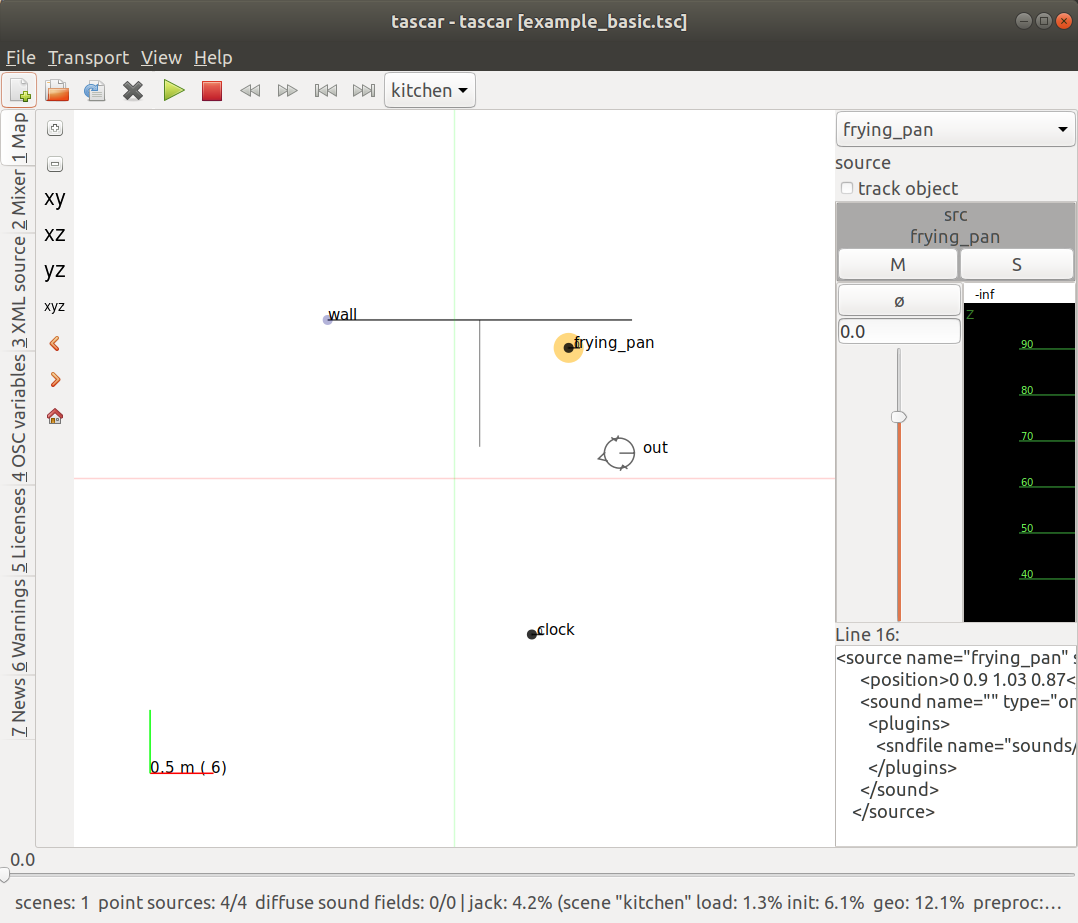
\includegraphics[width=0.4\textwidth]{tascarpro_mainwindow.png}
    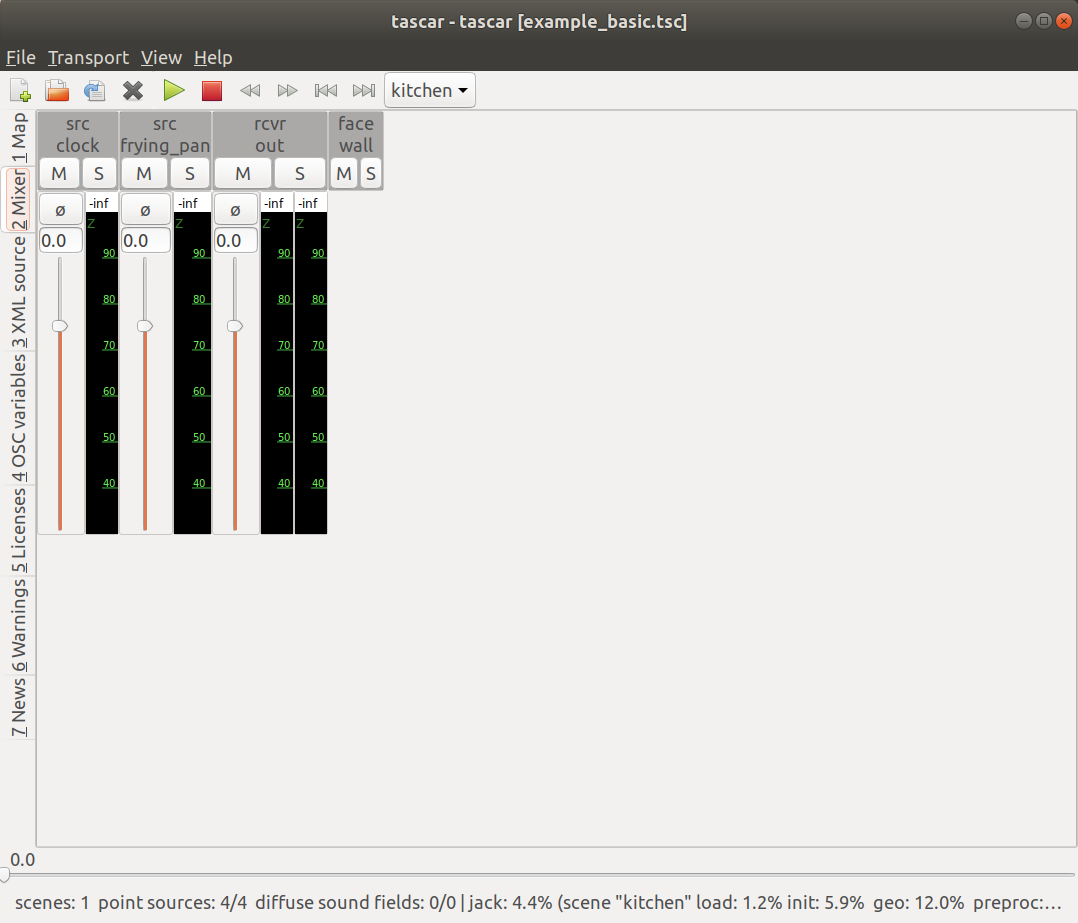
\includegraphics[width=0.4\textwidth]{tascarpro_mixer.png}\\
    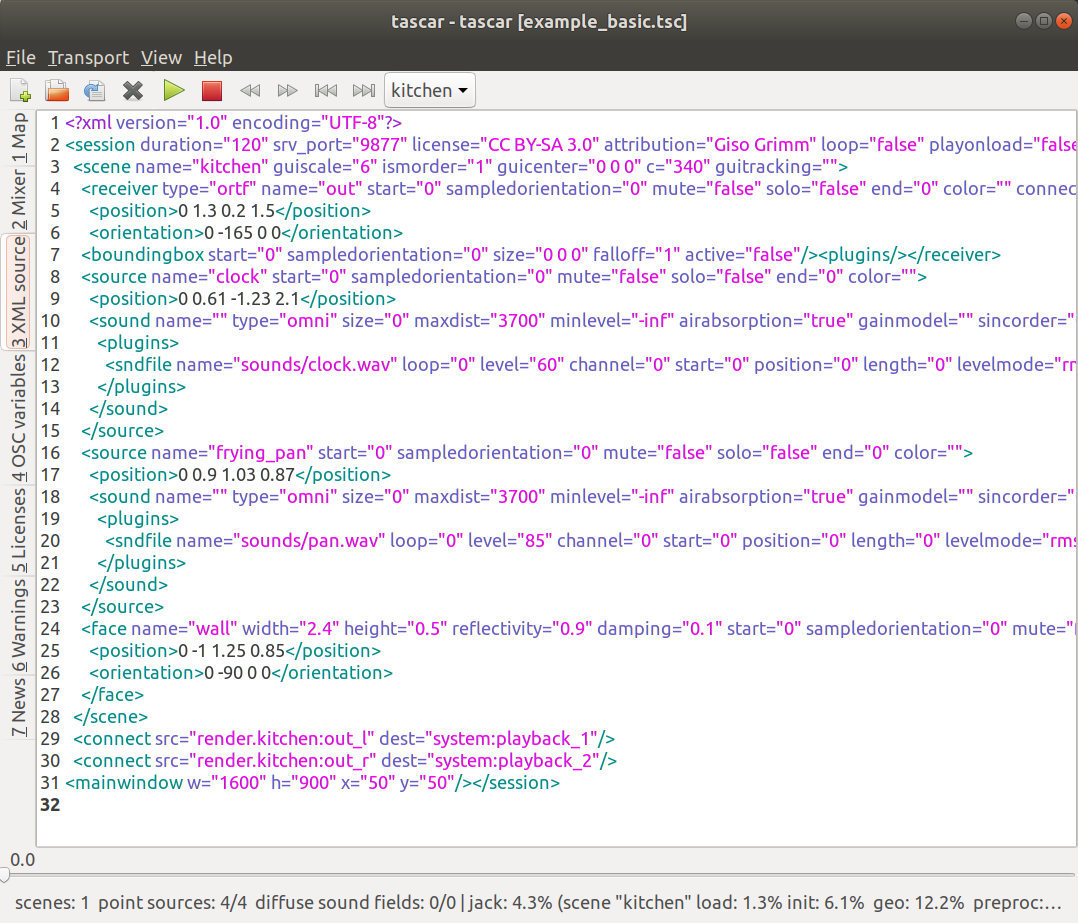
\includegraphics[width=0.4\textwidth]{tascarpro_xmlsource.png}
    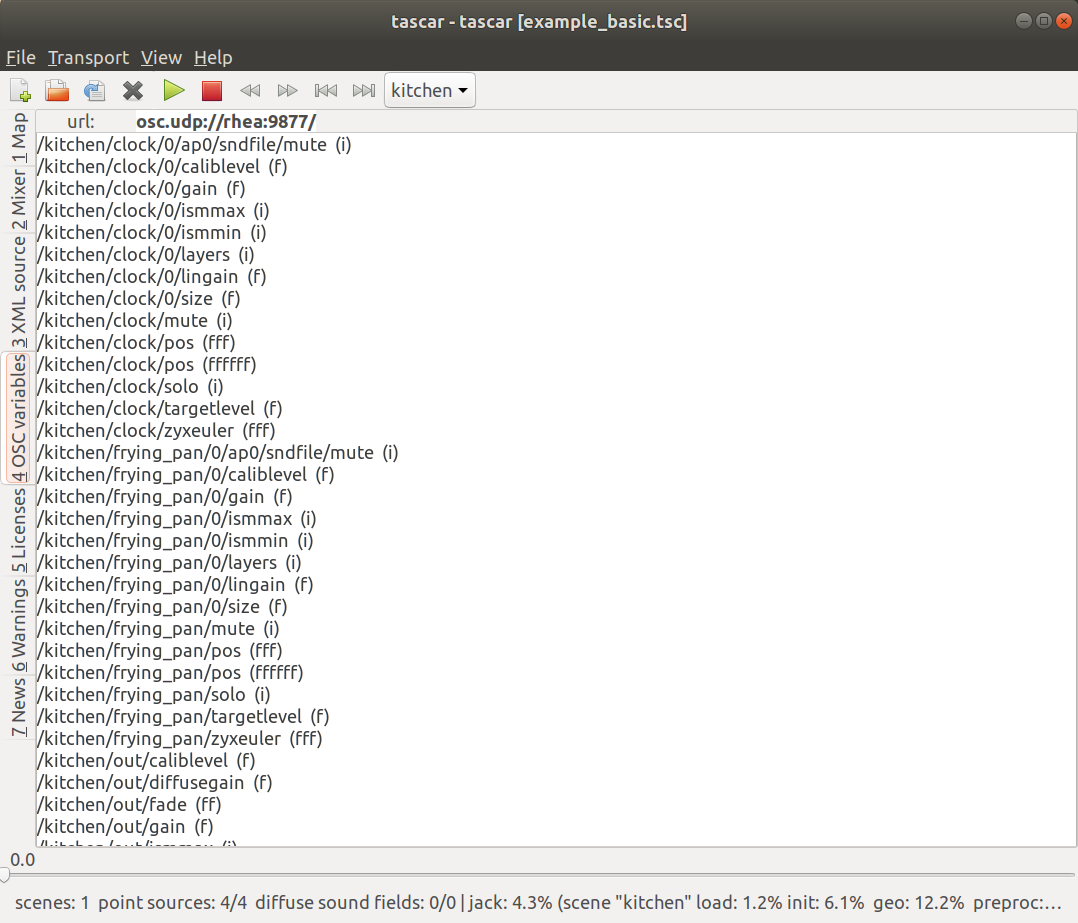
\includegraphics[width=0.4\textwidth]{tascarpro_osc.png}
    \caption{Example of some main window tabs in \tascar{}.}
    \label{fig:tascar_tabs}
\end{figure}

\subsection{Network remote control via OSC}

For remote control of most options, the Open Sound Control (OSC)
protocol can be used.
%
\tascar{} supports UDP and TCP transport.
%
If more than one transport layer or multiple ports are required, the
module ``oscserver'' (see Section \ref{sec:oscserver}) can be used.
%
A MATLAB/GNU Octave tool for remote control is available, see section
\ref{sec:sendosc} for more details.


\subsection{Optimization of the operating system for audio processing}

Configure real-time scheduling: grant permissions to acquire real-time
priority, and to lock memory in RAM, to users in group 'audio' (edit
{\tt /etc/security/limits.conf} as root):

\begin{verbatim}
sudo gedit /etc/security/limits.conf
\end{verbatim}

\begin{verbatim}
@audio - rtprio	 99
@audio - memlock unlimited
\end{verbatim}

Add desired user of tascar (in this example, this user is named 'tascar')
to group 'audio':
\begin{verbatim}
sudo adduser tascar audio
\end{verbatim}
Log out and log in again (no re-boot required).


After every login, deactivate CPU frequency scaling in BIOS, or switch
to maximum performance manually, e.\,g., with
\begin{verbatim}
for c in {0..11}; do cpufreq-selector -c $c -g performance; done
\end{verbatim}
or with the \tascar{} provided wrapper \verb!tascar_cpufreq!.

\subsection{Overwriting application default values}\label{sec:globalconfig}

Some variables which do not directly affect the acoustic rendering
result, e.g., GUI parameters and configuration of the loudspeaker
calibration tool, have built-in default values.
%
These values can be overwritten using an external application
configuration file in XML format. The files
\verb!/etc/tascar/defaults.xml! and \verb!${HOME}/.tascardefaults.xml!
  are read in this order, i.e., values in the second file overwrite
  the system defaults. To see the configurable variables, set the
  environment variable \verb!TASCARSHOWGLOBAL! to ``yes'' start the
  application from the command line, e.g.,
\begin{verbatim}
TASCARSHOWGLOBAL=yes tascar
\end{verbatim}
or
\begin{verbatim}
TASCARSHOWGLOBAL=yes tascar_spkcalib
\end{verbatim}
%
An example application configuration file can look like this:
\begin{verbatim}
<tascar>
  <spkcalib>
    <inputport data="system:capture_29"/>
    <reflevel data="80"/>
  </spkcalib>
</tascar>
\end{verbatim}
%
This will translate into these variables:
\begin{verbatim}
tascar.spkcalib.inputport (system:capture_29)
tascar.spkcalib.reflevel (80)
\end{verbatim}

\subsection{Content ownership rights}

Complex virtual acoustic or audiovisual environments in \tascar{}
often depend on a huge amount of external files, e.g., sound files,
trajectory data, 3D models, or texture and material definitions.
%
Keeping track of the ownership of many files can be difficult.
%
Therefore, \tascar{} provides methods to facilitate the process of
fair and legally correct distribution of \tascar{} session files.
%
Part of these methods is the setting of authorship and license
abbreviations of session files (see Section \ref{sec:session}), and a
simple text file based way of specifying license conditions of
external sound files (see \ref{sec:ap_sndfile}).
%
A summary of the licenses used by a session is provided in the main
window in the ``Licenses'' tab and with the command line tool
\verb!tascar_showlicenses!.
%
Please always check the information provided by those tools carefully
before sharing a session file.

Please note that in many cases it is illegal to remove or modify
authorship and license information from files originating from other
sources.

\section{Scene Definition}

Acoustic scenes are created using XML scene definition file
format\index{file format}. \tascar{} scene definition (\verb!.tsc!-file) is a text XML
file, where the user specifies all the details about the scene using
various commands (elements and their attributes). An example of a
scene definition is shown below (example file \verb!example_basic.tsc!):
\tscexample{example_basic}

\refelem{scene}, \refelem{receiver}, \refelem{face},
\refelem{source} etc.\ are the elements and \textbf{name},
\textbf{loop}, \textbf{reflectivity}, \textbf{width} etc.\ are their
attributes. Figure \ref{fig:tascar_scene_example} shows the
representation of this scene definition in \tascar{}.
%
The main window\index{main window} contains a toolbar for file
interactions, transport and time control, and controls for muting and
soloing the different components of the scene (left panel).
%
The scene map window contains a visual representation of the
scene. Editing the scene via the graphical user interface is currently
not possible.

\begin{figure}[htb]
    \centering
    \fbox{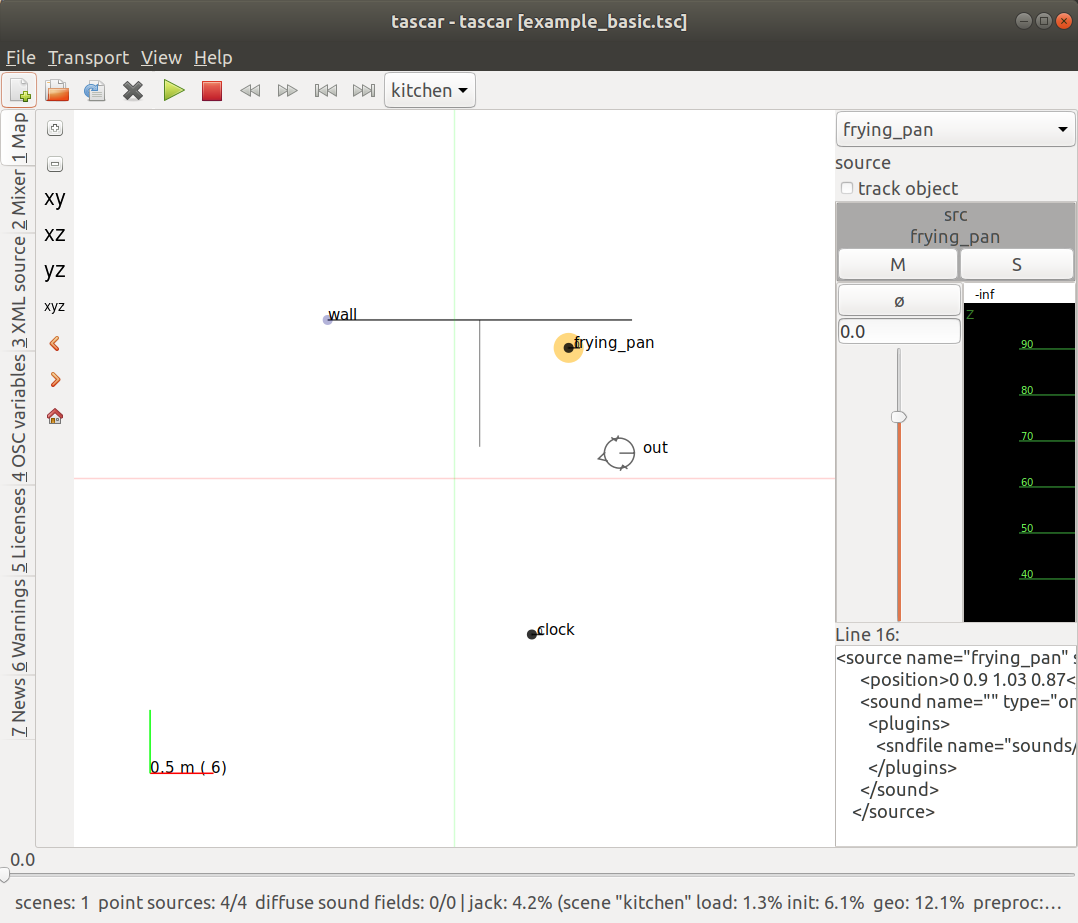
\includegraphics[width=\textwidth]{tascarpro_mainwindow.png}}
    \caption{Simple \tascar{} scene example. Scene consist of two sources, one reflector and one receiver. }
    \label{fig:tascar_scene_example}
\end{figure}

%\framebox[1.1\width]{\textbf{tascar example\_ktchen.tsc}} \\

Note: In general, if an attribute or a element is not specified in
the scene definition, it is set to default. Therefore, it is not
necessary to specify all the recognized attributes and elements.

\section{Top level elements}

Elements \refelem{session} and \refelem{scene} are referred to as
top-level elements in \tascar{} documentation.
%
One \refelem{session} element can contain multiple \refelem{scene}
elements.
%
Together, they form the outermost building blocks of \tascar{} scenes.

\subsection{The {\tt <session>...</session>} element}\label{sec:session}\index{session}

\elem{session} is the root element of each scene definition file. It
can contain one or more scenes (\refelem{scene}), port connections
(\elem{connection}), external modules (\elem{modules}) and range
definitions (\elem{range}).

\input{tabsession.tex}

\begin{tscattributes}
\indattr{name}               & Name of session (default: ``tascar'')                                                           \\
\indattr{duration}           & Duration of session in seconds; default: 60                                                     \\
\indattr{loop}               & Loop session (true|false); default: false                                                       \\
\indattr{playonload}         & Start playback when loading the session (true|false); default: false                            \\
\indattr{levelmeter\_tc}     & Level meter time constant in seconds; default: 2                                                \\
\indattr{levelmeter\_weight} & Level meter weight type; default: Z (``Z'', ``C'' or ``bandpass'')                              \\
\indattr{levelmeter\_min}    & Level meter minimum in dB (default: 30)                                                         \\
\indattr{levelmeter\_range}  & Level range of level meters in dB (default: 70)                                                 \\
\indattr{levelmeter\_mode}   & Level meter mode (rms, rmspeak, percentile)                                                     \\
\indattr{srv\_addr}          & OSC server multicast address, empty uses unicast                                                \\
\indattr{srv\_port}          & OSC server port number (default: 9877), or ``none'' to deactivate OSC server                    \\
\indattr{srv\_proto}         & OSC server protocol (default: ``UDP'', options are ``UDP'' or ``TCP'')                          \\
\indattr{warnsrate}          & Session sampling rate in Hz, print a warning if the system sampling rate doesn't match          \\
\indattr{requiresrate}       & Session sampling rate in Hz, stop loading the session if the system sampling rate doesn't match \\
\indattr{warnfragsize}       & Session fragment size, print a warning if the system fragment size doesn't match                \\
\indattr{requirefragsize}    & Session fragment size, stop loading the session if the system fragment size doesn't match       \\
\indattr{initcmd}            & Command to be executed before first connection to jack. Can be used to start jack server.       \\
\indattr{initcmdsleep}       & Time to wait for initcmd to start up, in seconds.                                               \\
\indattr{license}            & License form of session file                                                                    \\
\indattr{attribution}        & Attribution of session file, e.g., author name                                                  \\
\indattr{starturl}           & URL to display in news tab (default: http://news.tascar.org/)                                   \\
\end{tscattributes}

The sampling rate and fragment size of a session is typically defined
by the jack server or the interface of the offline rendering
tools. Use the attributes \attr{warnrate}, \attr{requiresrate},
\attr{warnfragsize} and \attr{requirefragsize} for more control over
the audio back-end settings.

A session can have sub-elements \elem{mainwindow} and \elem{mapwindow}
to control the window positions. These attributes are allowed:
\begin{tscattributes}
\indattr{x} & x-position of window            \\
\indattr{y} & y-position of window            \\
\indattr{w} & Width of window (default: 1600) \\
\indattr{h} & Height of window (default: 480) \\
\end{tscattributes}

An example of a session with multiple scenes is:
\tscexample{example_multiplescenes}

The jack transport can be controlled via the OSC paths {\tt
  /transport/start}, {\tt /transport/stop} and {\tt
  /transport/locate}.

A special sub-element \elem{include} can be used to include scenes
and other elements from another session file, given by the attribute
\indattr{name}. Example:
\begin{lstlisting}[numbers=none]
<?xml version="1.0"?>
<session>
  <include name="session1.tsc"/>
  <include name="session2.tsc"/>
</session>
\end{lstlisting}
\begin{tscattributes}
\indattr{name}        & File name to be included                       \\
\indattr{license}     & License form of session file                   \\
\indattr{attribution} & Attribution of session file, e.g., author name \\
\end{tscattributes}

The \elem{include} element can also be used at other levels; the
only limitation is that the root element of the included file needs to
match the active element into which the external file is included.
%
In the example above, the root XML element of files
{\verb!session1.tsc!} and {\verb!session2.tsc!} has to be a
\refelem{session} element.
%
Any attributes of the root element in the included file
are ignored.
% Comment: This is counter-intuitive.  It is probably a hack to allow
% included files to allow multiple scenes (XML permits only a single
% root element).

The element \elem{license} can be used to specify additional licenses, e.g., for additional visual content.
In addition to the licenses, the authors can be specified using the \elem{author} element, and a bibliography can be provided using the \elem{bibitem} elements:
\begin{lstlisting}[numbers=none]
<session license="CC BY-SA 3.0" attribution="Author1">
  <license name="visuals" license="CC BY-SA-NC 3.0" attribution="Author2"/>
  <author name="Author1" of="audio"/>
  <author name="Author2" of="visuals"/>
  <bibitem>Grimm, G., Kollmeier, B., &amp; Hohmann, V. (2016). Spatial acoustic scenarios in multichannel loudspeaker systems for hearing aid evaluation. Journal of the American Academy of Audiology, 27(7), 557-566.</bibitem>
  ...
</session>
\end{lstlisting}
When at least one author is specified, then this information will be
displayed while loading the session.
%
Please note that in many cases it is illegal to remove or modify the
authorship information from a work, or change the original license
conditions.
%
Therefore it is possible in \tascar{} to specify multiple
\elem{author} and \elem{license} elements, to correctly attribute your
contributions to a session originating from other sources.


The file names provided in the name attribute of the \elem{include}
element can be absolute or relative.
%
Relative file names are relative to the directory containing the root
\verb!.tsc!-file.
% Comment: This is achieved by changing the current working directory
% (CWD) of the tascar process before loading a .tsc file using the
% gui.  Tobias considers this to be a bug.  Relative paths should
% either be relative to the unaltered CWD of the tascar process as on
% startup, or they should be relative to the file containing the
% respective <include> element.

\subsection{The {\tt <scene>...</scene>} element}\label{sec:scene}\index{scene}

\input{tabscene.tex}

\begin{tscattributes}
\indattr{name}        & Name of scene (default: ``scene'')                        \\
\indattr{guiscale}    & Display scaling in meter; default: 200                    \\
\indattr{guicenter}   & Display center (x, y, z) in meter; default: 0 0 0         \\
\indattr{guitracking} & Track an object in the scene map (default: use guicenter) \\
\indattr{ismorder}    & Order of image source model (default: 1)                  \\
\indattr{c}           & Speed of sound in m/s; default: 340                       \\
\indattr{active}      & Control activity of a whole scene (default: true)         \\
\end{tscattributes}

\begin{tscelements}
\refelem{source}, \refelem{receiver},
\refelem{diffuse}, \refelem{face}, \refelem{facegroup},
\refelem{obstacle}, \elem{description}
\end{tscelements}

\elem{scene} is a top-level element of a \tascar{} scene
definition. An example scene definition is given in Example
\ref{tsc:example_basic}.

\section{Objects}

A scene can be complemented with objects\index{object} of different types (as it was
already shown in the first example of a scene definition).
%
Objects can be any of the following types:
\begin{itemize}
\item sources (\refelem{source}), diffuse sound fields (\refelem{diffuse})
\item receivers (\refelem{receiver})
\item reflectors (\refelem{facegroup}, \refelem{face})
\item obstacles (\refelem{obstacle})
\item masks (\refelem{mask})
\end{itemize}
There can be many objects of different types in the scene. Each object
has position and orientation in space and time, and may also contain
different attributes depending on the type.

There are two different ways of defining the position and orientation
of an object - ``interactive'' and ``not interactive''.
%
First, we have to specify the ``not interactive'' position and
orientation (it can be also the whole trajectory of an object) in a
scene definition file.
%

As an addition to this predefined geometry, we can steer the object
using an external device, for example a joystick, head movement
tracking system or by an algorithm which generates a certain type of
movement, thus applying ``interactive'' type of geometry.
%
The resulting position and orientation of an object will be calculated
by summing up these two mentioned types of position and
orientation.
%
The difference between two types of defining the movement has been
depicted in Figure \ref{fig:positions}.

\begin{figure}[htb]
  \centering
  \fbox{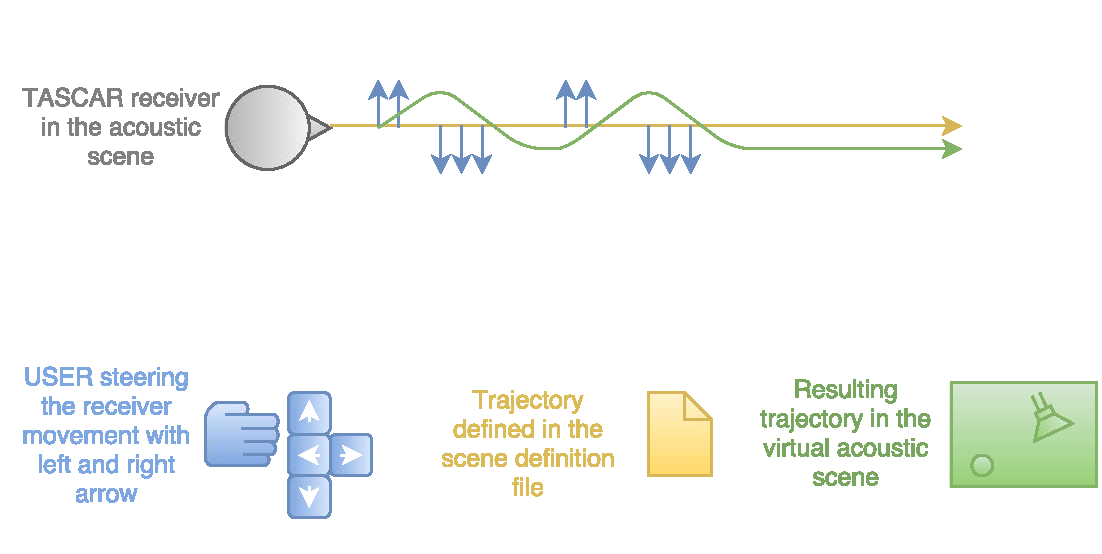
\includegraphics[width=0.8\textwidth]{positions}}
  \caption{Two different ways of dealing with orientation and position in \tascar{}
}
  \label{fig:positions}
\end{figure}



\subsection{Common attributes of objects}
\label{common attributes}

The following attributes are common to all scene objects:

\begin{tscattributes}
\indattr{name}               & Name of the object (default: "in" for {\tt source}, "out" for {\tt receiver})                                                         \\
\indattr{mute}               & Mute the object; {\tt mute="true"} or {\tt mute="false"}; default: "false"                                                            \\
\indattr{solo}               & Solo the object (i.\,e.\ mute all objects which don't have solo activated); {\tt solo="true"} or {\tt solo="false"}; default: "false" \\
\indattr{color}              & Color of the graphical representation of the object (hex triplet)                                                                     \\
\indattr{start}              & Render activity start time in seconds; default: 0                                                                                     \\
\indattr{end}                & Render activity start time in seconds; default: 0                                                                                     \\
\indattr{localpos}           & Local position in meters (Cartesian coordinates); default: ``0 0 0''                                                                  \\
\indattr{sampledorientation} & Sample orientation along trajectory with this distance (default: 0)                                                                   \\
\indattr{dloaction}           & Delta location in meters (Cartesian coordinates); default: ``0 0 0''                                                                  \\
\indattr{dorientation}           & Delta orientation in degrees (ZYX Euler transformation); default: ``0 0 0''                                                                  \\
\end{tscattributes}

The delta transformation values can be overwritten by actor modules or
the OSC interface. The \attr{dorientation} attribute is first rotation
around Z axis, then Y axis, followed by X axis.

The render activity is limited to the interval [start,end] only if end
\(>\) start. All time information of objects, such as dynamic geometry
or sound file positions, are relative to the object start time.
%
This {\em object time} is defined as session time minus object start time.

Muting an object disables it, i.\,e., muting a \verb!source! will
disable the sound, muting a \verb!receiver! will disable the output of
the receiver, and muting a \verb!face! or \verb!facegroup! will
disable all image sources generated by that reflector.


\subsection{Common sub-elements of objects}

All scene objects (e.g. instances of
\refelem{source}, \refelem{receiver}, \refelem{mask},
\refelem{facegroup}, \refelem{face}, etc.) have to define their
position and orientation in space and time.
%
The following child elements can be used to specify these parameters
(see also Example \ref{tsc:example_basic}).

\subsubsection{The {\tt <position>...</position>} element}\label{sec:position}\index{position}

Position is specified by providing Cartesian coordinates (in meters)
as well as the time point associated with them (object time in
seconds, counted with respect to the time when the object starts to be
active, see attribute \attr{start} of parent element):
\itscexamplepriv[linerange={1-1},numbers=none]{pos_and_rot}

If we want the object to change its position over the course of the
scene, we have to specify more than one point in space and time:
%
\itscexamplepriv[linerange={3-7},numbers=none]{pos_and_rot}
t\_n is time and x\_n, y\_n and z\_n are the Cartesian coordinates of
an object at time t\_n.  The object's position will be linearly
interpolated between these points.
%
The numbers are separated by white space.
%
The line breaks in this example are solely for human readability,
and not required by the \tascar{} software.

We can also use an attribute to control the interpolation method:
\itscexamplepriv[linerange={9-16},numbers=none]{pos_and_rot}
The first example will interpolate linearly in Cartesian coordinates,
i.\,e., the object will move on a straight line from (1,4,0) to
(1,-4,0).
%
The second example will interpolate linearly in spherical coordinates
around the origin, i.\,e., the object will move along an arc from
(1,4,0) to (1,-4,0).

The last position of the position track is held until the either the
session, or the current position loop iteration (see below),
terminates.

Instead of defining the position track in the tsc file it can also be
read from a comma-separated file, by setting the attribute
\indattr{importcsv}. Please note that the file needs to be comma
separated, with four numbers $t,x,y,z$ in each row.
%
\begin{lstlisting}[numbers=none]
  <position importcsv="myfile.csv"/>
\end{lstlisting}

Position tracks and orientation tracks can be looped by adding the
attribute \indattr{loop} with a number larger than zero.

\begin{lstlisting}[numbers=none]
  <position loop="10">0 0 0 0
  6 10 0 0</position>
\end{lstlisting}

in this case, the position/orientation is sampled with the object time
modulo loop time (10 seconds), i.\,e., the object is moving for 6
seconds, then resting at (10,0,0) for 4 seconds, then again moving for
6 seconds, starting at (0,0,0).

\begin{tscattributes}
  \indattr{interpolation}
  &
  Coordinate system in which positions are linearly interpolated
  between given positions. Possible values are {\tt cartesian} and
  {\tt spherical}. Default: {\tt cartesian}.
  \\
  \indattr{importcsv}
  &
  Read position track from the \verb!.csv!-file as
  comma-separated values.  The file name can contain absolute or
  relative path.  Relative paths are relative to the session's
  \verb!.tsc!-file. Default: position track is contained as
  space-separated text between opening and closing \refelem{position}
  tags.
  \\
  \indattr{loop}
  &
  The value, if greater than {\tt 0}, specifies the time in seconds
  when this position track is repeated from {\tt 0}. Default: {\tt 0},
  no repetition.
  \\
\end{tscattributes}

\subsubsection{The {\tt <orientation>...</orientation>} element}\label{sec:orientation}\index{orientation}

Orientation is specified in Euler (navigation) angles $R_{z,y,x}$, measured in degrees:
%
\itscexamplepriv[linerange={18-18},numbers=none]{pos_and_rot}
$R_z$ is the rotation around the z-axis, $R_y$ around the y-axis and
$R_x$ around the x-axis. They are applied in z,y,x order, after
application of the position.
%
If we would like the orientation of an object to change during the
scene, we can specify multiple angles and time points associated with
them:
\itscexamplepriv[linerange={20-23},numbers=none]{pos_and_rot}
%
The numbers are separated by white space.
%
The line breaks in this example are solely for human readability,
and not required by the \tascar{} software.

The last orientation of the orientation track is held until the either
the session, or the current orientation loop iteration (see below),
terminates.

Instead of defining the orientation directly in the tsc file it can
also be read from a comma-separated file, by setting the attribute
\indattr{importcsv}.

Euler orientation tracks can be looped by adding the attribute
\indattr{loop} with a number larger than zero.

\begin{tscattributes}
  \indattr{importcsv}
  &
  Read orientation track from the \verb!.csv!-file as
  comma-separated values.  The file name can contain absolute or
  relative path.  Relative paths are relative to the session's
  \verb!.tsc!-file. Default: orientation track is contained as
  space-separated text between opening and closing
  \refelem{orientation} tags.
  \\
  \indattr{loop}
  &
  The value, if greater than {\tt 0}, specifies the time in seconds
  when this orientation track is repeated from {\tt 0}. Default:
  {\tt 0}, no repetition.
  \\
\end{tscattributes}

\subsubsection{The {\tt <creator>...</creator>} element}\label{sec:creator}\index{creator}

Instead of defining the object's movement manually (defining position
and orientation for each time point) we can use the creator tool.
\tscexamplepriv[linerange={8-14},firstnumber=8]{example_cashdesk} In
this case, the orientation is calculated as a tangent along the given
path.

\subsubsection{Delta-transformations}\label{sec:deltatransform}\index{delta-transformation}

In addition to the transformation defined by the \elem{position},
\elem{orientation} and \elem{creator} elements, every object has a
delta-transformation which can be controlled via OSC or by actor
modules (see section \ref{sec:actormod}).

\subsubsection{The {\tt <navmesh/>} element}\label{sec:navmesh}\index{navmesh}\index{navigation mesh}

The navmesh element can be used to restrict the object motion to a
navigation mesh.
%
This is specifically useful when controlling object positions via game
controllers.

\begin{tscattributes}
\indattr{importraw} & File name of raw file containing list of polygon surfaces. \\
\indattr{maxstep}   & Maximal vertical step size.                                \\
\indattr{zshift}    & Vertical shift of control position, to achieve
above-floor positions with a floor navigation mesh.                              \\
\end{tscattributes}

Faces can be imported from a text file, containing space-separated
lists of polygon coordinates (see section \ref{sec:facegroup} on face
groups for details), or within the \elem{faces} sub-element.

\subsection{The {\tt <source>...</source>} element}\label{sec:source}\index{source}

\underline{Recognized attributes:}

\refelem{source} supports the attributes common to
all scene objects, refer to section \ref{common attributes}
\nameref{common attributes} on page \pageref{common attributes} for
details.

\input{tabsource.tex}

\underline{Recognized sub-elements:}

\refelem{position}, \refelem{orientation}, \refelem{creator}, \refelem{sound}

\elem{source} is an element used to create the sound source
objects in the scene definition. Since sources are also objects, they
can have a trajectory (see \ref{common attributes}).  A source
object can consist of one or more "sound vertices" specified with a
sub-element \refelem{sound}. There must also be a sound content, for
example from a sound file, assigned to a source. We can assign a sound
content to a source using the audio plugin
\refelem[ap_sndfile]{sndfile}.

In the box below we can see a definition of a simple point source
object (taken from Example \ref{tsc:example_basic}):
\tscexamplepriv[linerange={16-23},firstnumber=16]{example_basic}

\subsubsection{The {\tt <sound .../>} element}\label{sec:sound}\index{sound}\index{vertex}

\input{tabsound.tex}

\begin{tscattributes}
\indattr{type}                          & Sound source radiation type (default: ``omni'')                                            \\
\indattr{gainmodel}                     & Gain model, either ``1/r'' or ``1'' (default: ``1/r'')                                     \\
\indattr{size}                          & Physical size for source width simulation\footnote{Currently only used by receiver hoa2d.} \\
\indattr{sincorder}                     & Sinc interpolation order, 0 = nearest neighbor; default: 0                                 \\
\indattr{caliblevel}                    & Calibration level in dB; default: 93.9794                                                  \\
\indattr{gain}                          & Gain in dB; default: 0                                                                     \\
\indattr{x},\indattr{y}, \indattr{z}    & Local Cartesian coordinates in meter; default: 0                                           \\
\indattr{az},\indattr{el}, \indattr{r}  & Local spherical coordinates in degrees; default: use Cartesian                             \\
\indattr{rz},\indattr{ry}, \indattr{rx} & Local vertex Euler orientation in degrees; default: 0                                      \\
\indattr{d}                             & Chain distance (vertex distance along trajectory); default: 0                              \\
\indattr{maxdist}                       & Maximum delay line length in meter; default: 3700                                          \\
\indattr{minlevel}                      & Minimum SPL for source to be rendered (default: -inf)                                      \\
\indattr{ismmin}                        & Minimal ISM order to be rendered (0)                                                       \\
\indattr{ismmax}                        & Maximal ISM order to be rendered ($2^{32}$)                                                \\
\indattr{layers}                        & List of active layers, or empty for all layers (default)                                   \\
\indattr{airabsorption}                 & Render air absorption (default: true)                                                      \\
\indattr{name}                          & Name (suffix)                                                                              \\
\indattr{connect}                       & Jack port connection                                                                       \\
\end{tscattributes}

Another sub-element used in the example is \elem{sound}. With this
sub-element we specify the sound vertices of the source object, i.e.,
points from which the sound radiates.
%
Properties of the sound vertex define its radiation characteristics
(\attr{type}, \attr{gainmodel}, \attr{size}, \attr{sincorder}), its
level calibration and gain characteristics (\attr{caliblevel},
\attr{gain}), activity processing (\attr{maxdist}, \attr{minlevel},
\attr{layers}), image source model settings (\attr{ismmin},
\attr{ismmax}) and the relative position and orientation (\attr{x},
\attr{y}, \attr{z}, \attr{az}, \attr{el}, \attr{r}, \attr{rz},
\attr{ry}, \attr{rx}, \attr{d}). Please note that the local position
relative to the object origin and orientation can be provided either
in Cartesian coordinates (\attr{x}, \attr{y}, \attr{z}) or in
spherical coordinates (\attr{az}, \attr{el}, \attr{r}), however, these
can not be mixed.

If we want to create a point source, as in the example, we will
have one sound vertex exactly at the position of the source
object (so at the point specified in the element \elem{position}).
%
When we create a source with more than one
sound vertex, the object position specified in sub-element \elem{position}
will now be the reference point for all the sound vertices, and
changing this position will also change the position of the sound
vertices.
%
The same holds for the orientation of a source object consisting of
more than one sound vertex.
%
Below we can see how such a source has to be defined:

\tscexample[linerange={4-20},firstnumber=4]{example_vertices}

We have a source object called "audience" which is made of four sound
vertices called "guy1","guy2" etc.
%
Their position is specified relative to the position in the
sub-element \elem{position} using attributes \attr{x}, \attr{y}
and \attr{z} -- for example the vertex called "guy1" is located
-0.7\,m from the reference point in x direction and 0.1\,m in y
direction.

Figure \ref{fig:vertices} presents an example of a scene containing sound sources
consisting of more than one sound vertex.

\begin{figure}[htb]
  \centering
  \fbox{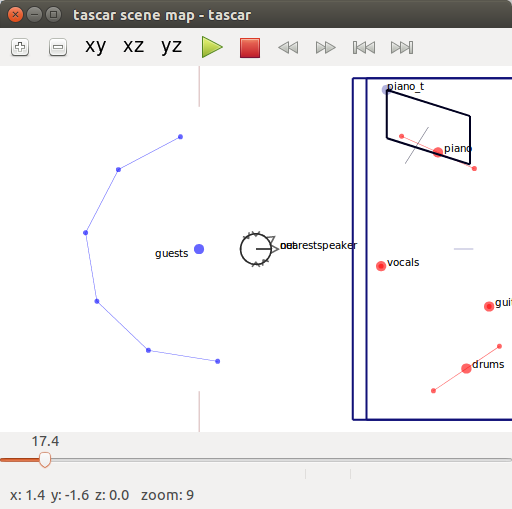
\includegraphics[width=0.8\textwidth]{jazzclub.png}}
  \caption{Examples of sound sources and their vertices. In this scene
    there are point sources like "vocals" or "guitar". There are also
    sound sources with more than one vertex like "guests" (6 vertices)
    or "piano" (2 vertices) - the big dot close to the name of the
    source is the reference point for a given source.}
  \label{fig:vertices}
\end{figure}

Source directivity is defined by the source module types. Currently
the types ``omni'', ``cardioidmod'' and ``door'' are supported.

Audio content can be added either from external playback (using jack
ports, see the \attr{connect} attribute), or using the audio plugin
\elem{sndfile} (see \ref{sec:ap_sndfile}). When recording new audio
material, we recommend to follow the documentation recommendations of
the DEGA \citep{dieter_leckschat_2020_3597238}. A useful source of
sound files can be found at \url{https://freesound.org/}.

\subsubsection{Source directivity ``omni''}

The ``omni'' source directivity has no configuration variables. The
sound source radiates independently of the direction.

\subsubsection{Source directivity ``cardioidmod''}

The ``cardioidmod'' source directivity has these attributes:
\begin{tscattributes}
\indattr{f6db} & Frequency in Hz, at which a 6~dB attenuation at 90 degrees is achieved (default: 1000) \\
\indattr{fmin} & Low-end limit for stabilization (default: 60)                                          \\
\end{tscattributes}
At low frequencies, the source radiates omni-directionally. At higher
frequencies, a cardioid-like radiation pattern is achieved.

\subsubsection{Source directivity ``door''}

The ``door'' source directivity has these attributes:
\begin{tscattributes}
\indattr{width} & Door width in meters (default: 1)\\
\indattr{height} & Door height in meters (default: 2)\\
\indattr{falloff} & Distance at which the gain attenuation starts (default: 1)\\
\indattr{distance} & Distance by which the source is shifted behind the door (default: 1)\\
\indattr{wndsqrt} & Flag to control von-Hann fall-off (false, default) or square-root of von-Hann fall-off (true)\\
\end{tscattributes}
Door sources shift the perceived source position behind a ``door''
shape, limited by the edges. They are basically designed for
interactive transitions between simulated rooms.

\subsection{The {\tt <diffuse .../>} element}\label{sec:diffuse}\index{diffuse}\index{diffuse}

\begin{tscattributes}
\indattr{connect} & Jack connection of ports.                                          \\
\indattr{gain}    & Output gain in dB                                                  \\
\indattr{size}    & Size of box in which the diffuse sound field is audible; default: 1 1 1 \\
\indattr{falloff} & Length of von-Hann ramp outside the box in m; default: 1            \\
\end{tscattributes}

\begin{tscelements}
\refelem{position}, \elem{boundingbox},\refelem{orientation}, \refelem{creator}, \elem{plugins}
\end{tscelements}

Apart of sound sources which consist of one or more sound vertices, we
also have a possibility to create diffuse sound fields which ``fill''
the space and are equally loud within a given volume (for example
isotropic babble noise in a cafeteria, or remote traffic).
%
We can define a diffuse sound field in the following way:
\tscexample[linerange={15-18},firstnumber=15]{example_cashdesk}
%What are the connections in this example?

Sound files used to create diffuse sound fields should contain 4 channels
(B format, FuMa normalization).
%
With attribute \attr{size="x y z"} we can specify the dimensions of
the box in which the diffuse sound field is audible.
%
To provide a smooth decay of the diffuse sound field, there is a von-Hann
ramp for the gain of the source outside the box.
%
The length of the ramp can also be specified using
\attr{falloff="..."}.
%
 As all other objects, diffuse sound fields also have position and
orientation, which refers to a position and orientation of the box.


If a port connection is provided (\attr{connect} attribute), then the
four renderer input ports (which are always generated with the diffuse
sound field: \verb!render.<scenename>:<objectname>.n!) are connected
to the audio player output ports \verb!@.0!, \verb!@.1!, \verb!@.2!
and \verb!@.3!, where ''@'' is \verb!player.<scenename>:<objectname>!
.
%


An example on how to add the \elem{addsndfile} audio plugin to a
diffuse sound field can be found below:
%
\tscexample[linerange={5-9},firstnumber=5]{example_diffuse}

The input signal of diffuse sound fields is the B-format (Furse-Malham
normalization, channel sequence ``wxyz''). For level metering, the RMS level
of the w-channel is taken.


\subsection{The {\tt <receiver .../>} element}\label{sec:receiver}\index{receiver}

A receiver\index{receiver} object can be imagined as a virtual
microphone\index{virtual microphone}\index{microphone}, which captures
the sound in the virtual space, and serves as an output of the virtual
acoustic environment.
%
The choice of the receiver type depends on the playback system and the
desired rendering method.
%
It captures the signal of all sound sources in the scene and computes
these signals according to its type.
%
We can route the output signals to playback system, e.g., loudspeakers
or headphones.

\input{tabreceiver.tex}

\begin{tscattributes}
\indattr{connect}      & Connection to jack port                                                                  \\
\indattr{gain}         & Gain of jack port in dB; default: 0                                                      \\
\indattr{type}         & Receiver type (see below for a list of receiver types)                                   \\
\indattr{volumetric}   & Size of box for volumetric rendering (x,y,z in m); default: 0 0 0                        \\
\indattr{avgdist}      & Average distance which is assumed inside receiver boxes, or 0 to use $(\frac18 V)^{1/3}$ \\
\indattr{point}        & Render point sources (true|false); default: true                                         \\
\indattr{image}        & Render image sources (true|false); default: true                                         \\
\indattr{ismmin}       & Minimal ISM order to be rendered (0)                                                     \\
\indattr{ismmax}       & Maximal ISM order to be rendered ($2^{32}$)                                              \\
\indattr{layers}       & List of active layers, or empty for all layers (default)                                 \\
\indattr{layerfadelen} & Fade length after layer activation or deactivation                                       \\
\indattr{diffuse}      & Render diffuse sound fields (true|false); default: true                                  \\
\indattr{diffusegain}  & Gain applied to diffuse sound fields in dB; default: 0                                   \\
\indattr{falloff}      & Length of von-Hann ramp in m, or -1 for normal distance model; default: -1               \\
\indattr{caliblevel}   & Calibration level in dB; default: 93.9794                                                \\
\indattr{delaycomp}    & Subtract this value from delay in delay line, in seconds (0)                             \\
\indattr{muteonstop}   & Do not render any sound when transport is stopped (default: false)                       \\
\end{tscattributes}

\begin{tscelements}
\refelem{speaker}, \elem{boundingbox}, \refelem{position},
\refelem{orientation}, \refelem{creator}
\end{tscelements}

A receiver encodes the signals of primary sources, image sources and
diffuse sound fields into a receiver type specific output format. Each
receiver owns one jack output port for each output channel $n$; the
number of channels $N$ depends on the receiver type and
configuration. The output signal of a receiver is
$\mathbf{z}(t)=\left(z_1\left(t\right),z_2\left(t\right),\dots,z_N\left(t\right)\right)$.

The receiver functionality can be split into a {\em panning} or
directional encoding of primary and image sources, and a {\em
  decoding} of first order Ambisonics diffuse signals:
\begin{equation}
\mathbf{z}(t) =
\underbrace{\sum_{k=1}^K \mathbf{w}(\mathbf{p}_{k,rel}) y_k(t)}_\text{panning} +
\underbrace{\sum_{l=1}^L \mathbf{D}\hat{\mathbf{O}}_{rec}\hat{\mathbf{O}}^{-1}_{src}\mathbf{f}_l(t)^T}_\text{diffuse decoding}
\end{equation}
In the panning part, the driving weights
$\mathbf{w}=(w_1,w_2,\dots,w_N)$ depend on the relative source
position in the receiver coordinate system,
$\mathbf{p}_{rel}=\mathbf{O}_{rec}^{-1}\left(\mathbf{p}_{src}-\mathbf{p}_{rec}\right)$. For
the definition of the receiver orientation matrix $\mathbf{O}_{rec}$
see Eq.\ \ref{eq:orientation} on page
\pageref{eq:orientation}. $y_k(t)$ is the output signal of the
acoustic model, i.e., distance-dependent gain and air absorption, for
the $k$-th source; $K$ is the number of all primary and image
sources. In the diffuse decoding part, $\mathbf{D}$ is the receiver
type specific first order Ambisonics decoding matrix,
\begin{equation*}
\mathbf{D} = \left(
\begin{array}{cccc}
  d_{1,w} & d_{1,x} & d_{1,y} & d_{1,z} \\
  \vdots    & \vdots  & \vdots  & \vdots  \\
  d_{n,w}  & d_{n,x} & d_{n,y} & d_{n,z}
\end{array}\right)\text{,}
\end{equation*}
and $\hat{\mathbf{O}}_{rec}$is the rotation matrix for first order
Ambisonics signals, to compensate the receiver orientation (see
Eq.\ \ref{eq:foarot}, page \pageref{eq:foarot}). $\mathbf{f}_l$ is the
first order Ambisonics signal of the $l$-th diffuse sound field; $L$ is the
number of all diffuse sound fields, including diffuse reverberation inputs.

For all speaker based receiver types, $D$ is a first order Ambisonics
decoder matrix, with optional speaker density compensation and
decorrelation filters. To achieve a $\max rE$-decoder, set the
attribute \indattr{xyzgain} to 0.707 for regular horizontal speaker
layouts and to 0.577 for regular 3D speaker layouts.  For Ambisonics
based receiver types, $D$ is a diagonal matrix.
%
By default, the decoded output of the first order Ambisonics rendering
is de-correlated using FIR all-pass filters to achieve diffuse sound
fields and avoid coloration artifacts (see \indattr{decorr} and
\indattr{decorr\_length} for details).

Figure \ref{fig:renderer} presents the typical connections in \tascar{}
and may help to visualize the role of the receiver.

\begin{figure}[htb]
  \centering
  \fbox{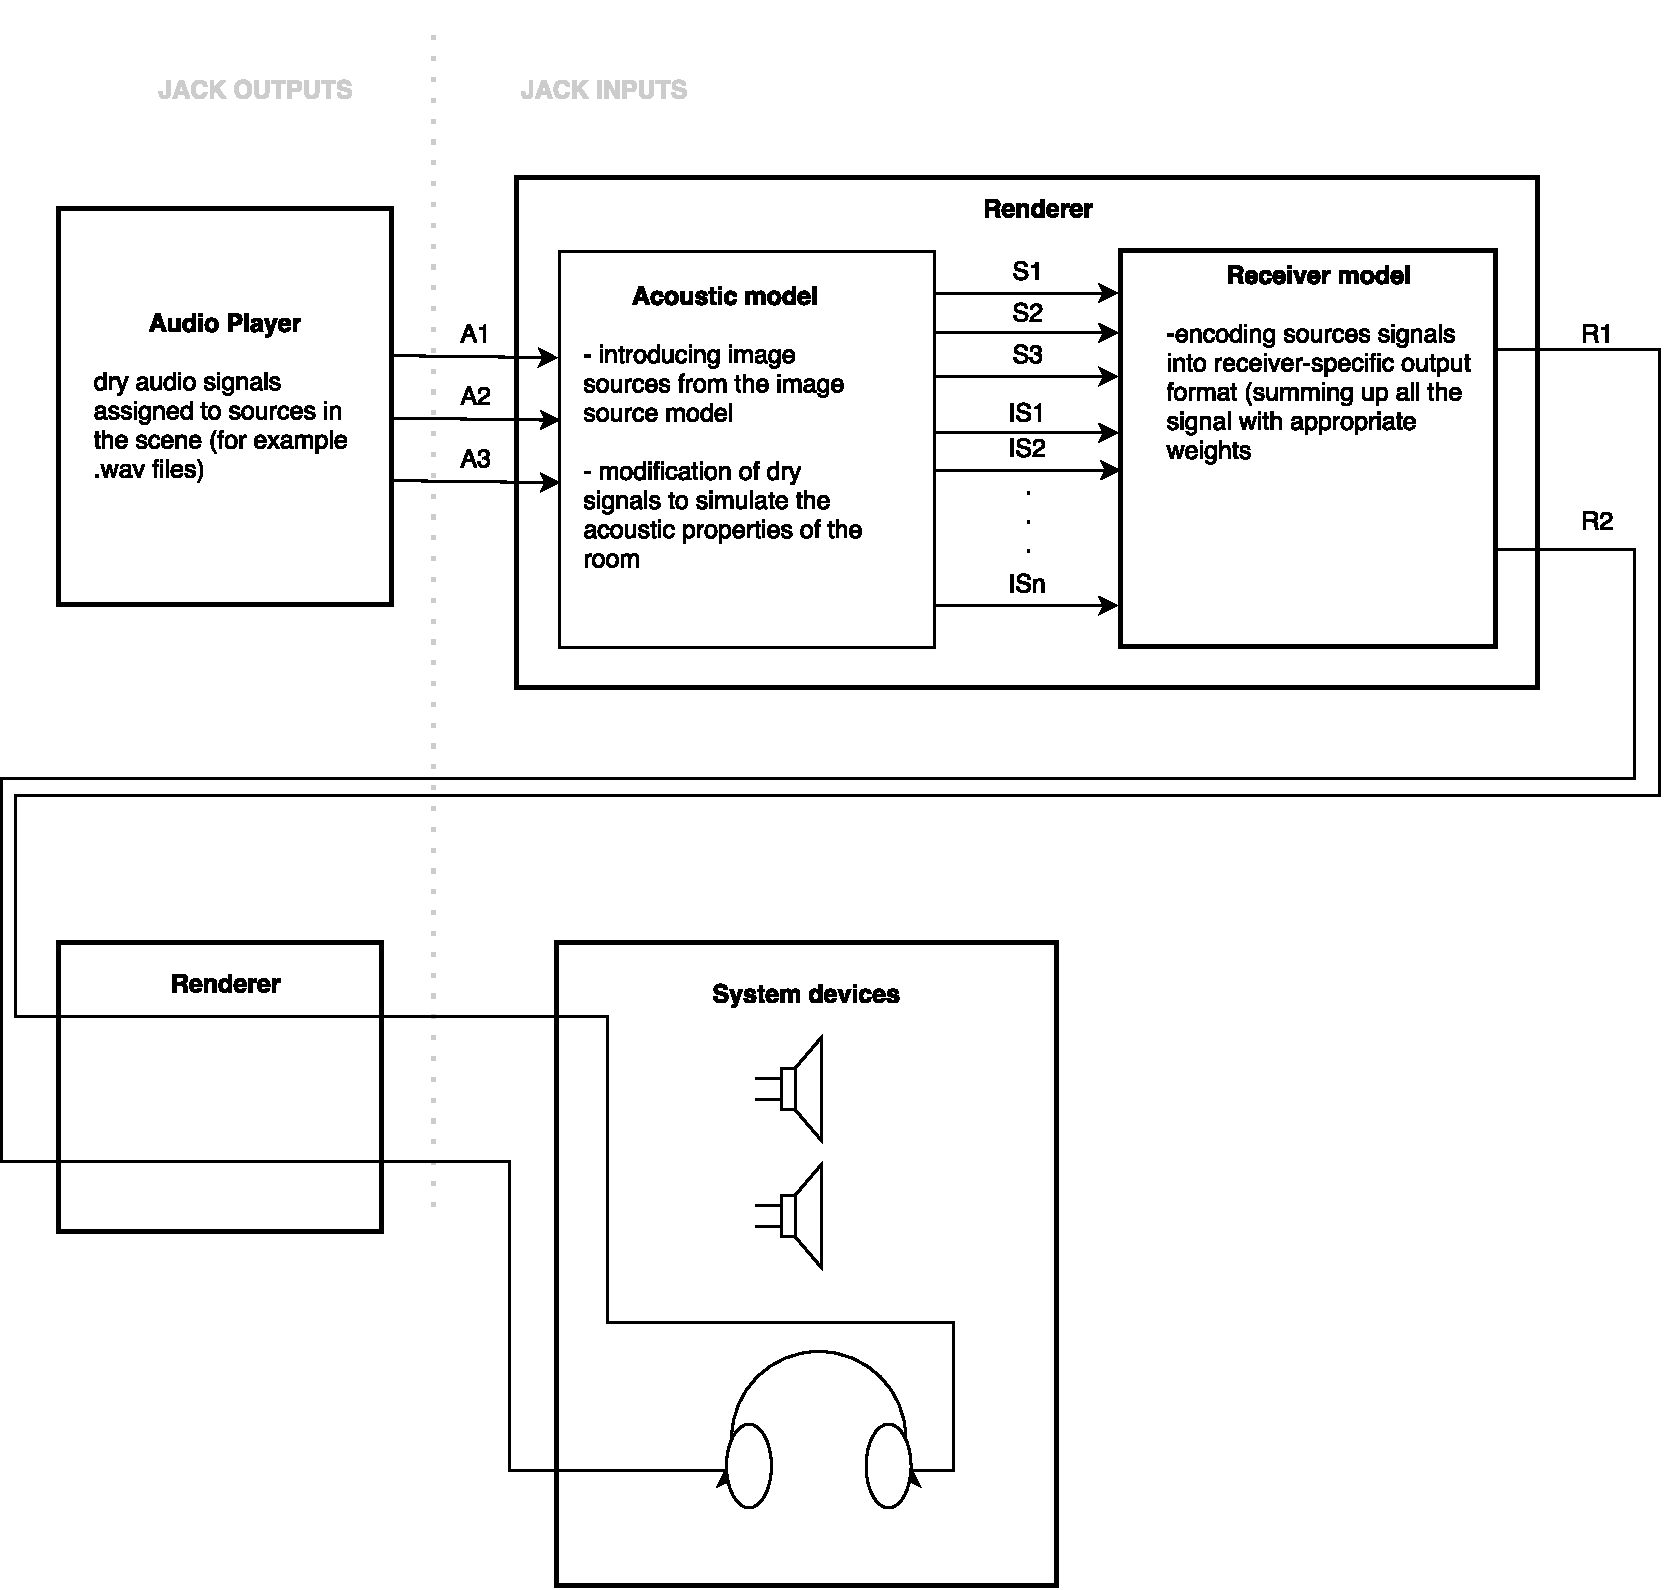
\includegraphics[width=0.8\textwidth]{renderer}}
  \caption{Typical structure of connections in \tascar{}.}
  \label{fig:renderer}
\end{figure}

If the \attr{volumetric}\index{volumetric rendering}\label{sec:volumetric}
attribute defines a non-zero volume, then all sources within the
receiver volume box are rendered with the same gain (volumetric
rendering).
%
An average distance of $(\frac18 V)^{1/3}$ with the volume $V$ is
assumed, or if \attr{avgdist} is provided, then the provided value is
taken.
%
Outside the box either a von-Hann ramp is applied (\attr{falloff}
$>0$), or the standard distance model is applied.
%
With volumetric receiver settings, the delay will depend on the
relative distance between the receiver origin and the source position.

%Example:
%
%\tscexample[linerange={5-12},firstnumber=5]{example_neukom}

\paragraph{OSC control}

Receivers can be controlled via OSC similar to other objects
(position, zyx Euler rotation, gain). They also support fade
commands:

\begin{verbatim}
/<scene>/<name>/fade <gain> <duration> [ <starttime> ]
\end{verbatim}
Here \verb!gain! is the linear target gain, \verb!duration! is the
length of the fade, and the optional third parameter \verb!starttime!
  is the start time, at which the fade is applied. If the current time
  is later than \verb!starttime! then the fade is applied
  immediately. The fade is always calculated using a raised cosine
  ramp. A new fade event will overwrite any currently ongoing or
  scheduled fade events.

\subsection{Receiver types}\index{receiver type}



There are following types of receivers (see Table \ref{tab:receivers} for an overview):

\input{secrecgeneric.tex}

\subsection{Speaker-based receiver types}\label{sec:speaker}\index{speaker}

There are also speaker-based decoding methods (VBAP, ambisonics
panning and nearest-speaker panning) which require the specification
of loudspeakers - together with the receiver type, we define a set of
virtual loudspeakers located relative to the position of this
receiver.
%
Information about the number of loudspeakers and their location is then
exploited to produce appropriate receiver output channels.
%

\begin{figure}[htb]
  \begin{subfigure}[t]{0.25\textwidth}
    \centering
    \fbox{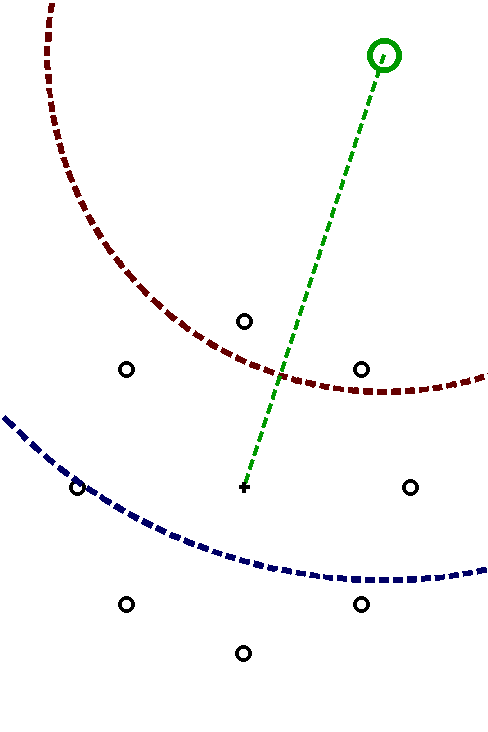
\includegraphics[width=0.85\linewidth]{method_input}}
    \caption{original}
  \end{subfigure}%
  \begin{subfigure}[t]{0.25\textwidth}
    \centering
    \fbox{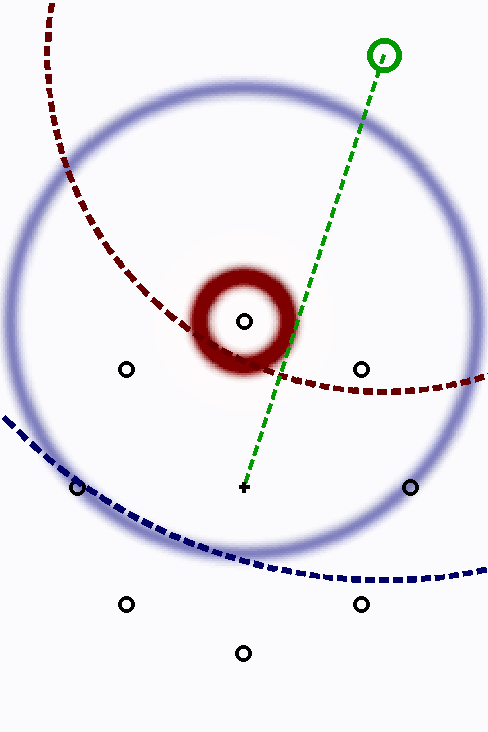
\includegraphics[width=0.85\linewidth]{method_nsp}}
    \caption{nsp}
  \end{subfigure}%
  \begin{subfigure}[t]{0.25\textwidth}
    \centering
    \fbox{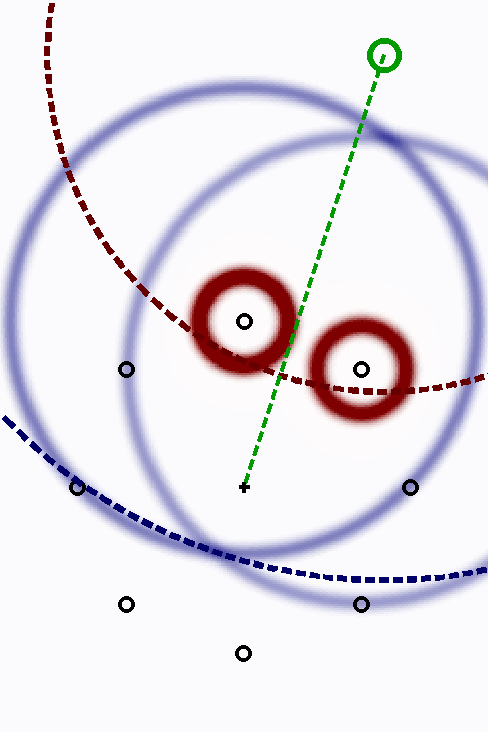
\includegraphics[width=0.85\linewidth]{method_vbap}}
    \caption{vbap}
  \end{subfigure}%
  \begin{subfigure}[t]{0.25\textwidth}
    \centering
    \fbox{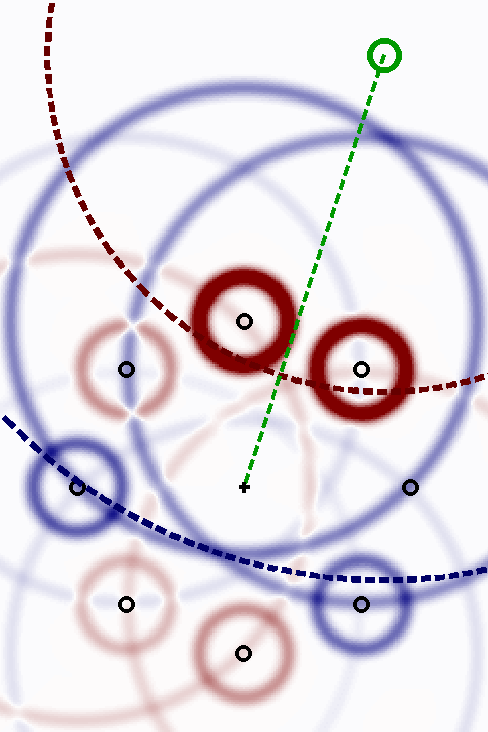
\includegraphics[width=0.85\linewidth]{method_amb_basic}}
    \caption{hoa2d}
  \end{subfigure}
  %\centering
  %\fbox{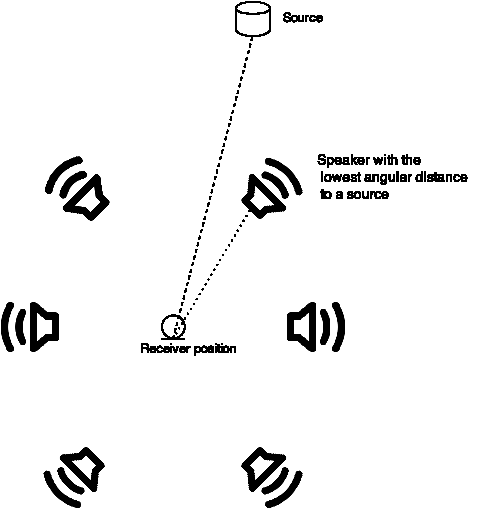
\includegraphics[width=0.8\textwidth]{nearest.pdf}}
  \caption{Schematic representation of the reproduced sound fields
    with different reproduction methods.}
  \label{fig:repromethods}
\end{figure}

The speaker layout of speaker based receiver types can be defined in a
separate layout file specified in the \attr{layout} attribute, in a
list of \elem{speaker} elements within the receiver definition.

\begin{tscattributes}
\indattr{az}      & Azimuth of loudspeaker in degrees (optional; default 0)   \\
\indattr{el}      & Elevation of loudspeaker in degrees (optional; default 0) \\
\indattr{r}       & Distance (optional; default 1)                            \\
\indattr{delay}   & Static delay in seconds (default: 0)                      \\
\indattr{label}   & Additional port label (optional; default empty)           \\
\indattr{connect} & Connection to jack port                                   \\
\indattr{compB}   & FIR filter coefficients for speaker calibration.          \\
\indattr{gain}    & Gain in dB (default: 0)                                   \\
\end{tscattributes}

In addition to regular broadband speakers, a number of subwoofers\index{subwoofer} can
be defined, using \elem{sub} elements with the same attributes as in
the \elem{speaker} element. If subwoofers are defined, an IIR
crossover filter is applied to all signals. Subwoofer signals are
spatially mapped from the broadband speaker positions to the subwoofer
positions, using a modified DBAP \citep{Lossius2009} method.

To activate FIR speaker correction filter, provide the FIR filter
coefficients in the \attr{compB} attribute. Please note that filter
coefficients are specific to the sampling rate, and not automatically
recalculated upon sampling rate changes. The maximal length of the
correction filter is the audio fragment size plus one.

The top-level element of a layout file, \elem{layout}, can be configured with these attributes:
\begin{tscattributes}
\indattr{caliblevel}     & Calibration level in dB; default: 93.9794                                           \\
\indattr{calibdate}      & Calibration date in format YYYY-MM-DD                                               \\
\indattr{xyzgain}        & XYZ-gain for FOA decoding                                                           \\
\indattr{decorr}         & Decorrelate speaker signals in diffuse sound field rendering (default: true)        \\
\indattr{decorr\_length} & Length of decorrelation filter, in seconds (default: 0.05)                          \\
\indattr{densitycorr}    & In diffuse rendering, correct gains locally for loudspeaker density (default: true) \\
\indattr{fcsub}          & Cross-over frequency in Hz, used only if subwoofers are defined (default: 80)       \\
\end{tscattributes}
%
Changing any of these attributes (except for \attr{calibdate}) might
affect the output calibration and requires re-calibration.

If the caliblevel is provided in the receiver element and the layout
file, then a warning is issued and the value from the layout file is
used. If a calibration date is provided and the calibration is older
than 30 days, a warning is displayed.


\input{secrecspeaker.tex}

\subsection{Adding diffuse reverberation: {\tt <reverb .../>}}\label{sec:reverbelem}

Diffuse reverberation can be added with the \elem{reverb} element. The
reverb plugin type is provided with the \attr{type} attribute, which
can be any of the types listed below.

Under the hood, the \elem{reverb} element combines a dedicated
receiver with a diffuse sound field. Therefore, most common attributes
of receivers (see \ref{sec:receiver}) can be used here as well. This
method of rendering diffuse reverberation is new to \tascar{} and
still under development. For the traditional way of creating diffuse
reverberation, see Section \ref{sec:reverb}. Advantages of the new
method over the old one are a much easier setup, and the full
functionality also for offline rendering.

A very basic FDN and a partitioned convolution module are provided as
part of \tascar{}. An example of diffuse reverberation using the
``simplefdn'' plugin looks like this:
%
\tscexample[linerange={35-37},firstnumber=35]{example_diffreverbnew}
%
The attribute ``volumetric'' defines the shoe-box shaped volume in
which sound sources are rendered. Diffuse sources do not contribute to
diffuse reverberation.

Reverb receivers have the attribute \attr{layers}, which defines the
layers in which the receiver receives sound, and \attr{outputlayers},
which defines the layers in which the diffuse sound field is
reproduced.

\input{secrecreverb.tex}

\subsection{Reflectors: {\tt <face .../>} and {\tt <facegroup .../>} elements}\label{sec:face}\label{sec:facegroup}\index{face}\index{facegroup}

The \elem{face} element defines a single reflecting surface.

\begin{tscattributes}
\indattr{width}, \indattr{height}         & Dimension of reflector in meters; default: 1                                       \\
\indattr{reflectivity}, \indattr{damping} & First order low pass filter coefficients                                           \\
\indattr{scattering}                      & Scattering coefficient (default: 0)                                                \\
\indattr{edgereflection}                  & Apply edge reflection in case of not directly visible image source (default: true) \\
\indattr{vertices}                        & List of Cartesian coordinates to define polygon surface                            \\
\end{tscattributes}

If the attribute \indattr{vertices} contains at least three
coordinates then a polygon surface is constructed using the vertices
list.
%
Otherwise, a rectangular surface with the given width and height is
created.
%
The vertices of the reflector are at $(0,0,0)$, $(0,w,0)$, $(0,w,h)$
and $(0,0,h)$. The face normal, i.e., the reflecting side of the
surface, is pointing in positive $x$-axis.

%
In \verb!example_reflectors.tsc! both cases are shown:
\tscexample[linerange={4-11},firstnumber=4]{example_reflectors}

The \elem{facegroup} element creates a group of polygon reflectors,
with common reflection properties.

\begin{tscattributes}
\indattr{reflectivity}, \indattr{damping} & First order low pass filter coefficients                                           \\
\indattr{importraw}                       & File name of raw file containing list of polygon surfaces                          \\
\indattr{shoebox}                         & Dimension of a shoebox shaped room with inward-facing walls (default: ``0 0 0'')   \\
\indattr{edgereflection}                  & Apply edge reflection in case of not directly visible image source (default: true) \\
\end{tscattributes}

Element \elem{facegroup} behaves also as an object, since it also has
a position and orientation in space.
%
So if we change the position or orientation of the whole
\elem{facegroup}, it will also relatively change for all the planes
included in the \elem{facegroup}.

We can define a \elem{facegroup} in the following way (see example
\verb!example_reflectors.tsc!):
\tscexample[linerange={12-17},firstnumber=12]{example_reflectors}

First, we define the facegroup with the name, reflectivity as well as
the position and orientation of the whole facegroup.
%
Then, we use a sub-element \elem{faces} (not the same as \elem{face}
!) to define the surfaces which will be included in the group.
%
Each line has to contain the coordinates x y z for at least three
vertices.
%
Each surface is defined in one line (by specifying coordinates of the
vertices of a surface).
%
At this point in the code we shouldn't leave empty lines.

Instead of defining all the surfaces manually, they can be modeled in
blender (blender 2.79 -- the scripts do not yet work with blender
2.80). The meshes can be exported with:
\begin{verbatim}
tascar_blenderexport blendfile.blend
\end{verbatim}
This will export the meshes of all blender mesh objects of the
currently selected scene, or if available, from the scene named
``tascar'', to the file {\tt <blendfilename>\_<objectname>.raw} and
all curve objects to a \tascar{} track file {\tt
  <blendfilename>\_<objectname>.csv}. Curve objects may set the custom
property ``speed'' (see ``Custom properties'' in the ``Object'' tab in
the blender property view), to set the speed in $m/s$.

It is recommended to minimize the number of faces, e.g. by using
polygon faces instead of triangulated faces. Also only the
acoustically relevant surfaces should be modeled, e.g. typically only
the top of a table is acoustically important, but a table modeled for
visualization also contains the bottom, legs and side surfaces.
%
If all these surfaces were imported into \tascar{}, one image source
would be created for each of the reflectors and primary sources, which
would lead to a waste of computational performance. Small structures
can be better modeled using the \attr{scattering} attribute of
reflectors. Late reverberation can be modeled independently of the
image source model (see Section \ref{sec:reverbelem}).

When we already have a text file, where the coordinates for all the
vertices are already specified, we can import it to \tascar{} scene
definition using an attribute \indattr{importraw}:
\begin{lstlisting}[numbers=none]
<facegroup name="mirrors" reflectivity="1" damping="0" importraw="filename.raw"/>
\end{lstlisting}

A simple shoebox shaped room can be created by setting the attribute
\attr{shoebox="x y z"} to a finite size.
%
The size is given in $x,y,z$ dimensions. All faces are pointing
inwards.

The normal of faces, i.e., the face orientation, is relevant for the
acoustics simulation: Image sources are only active if the primary
source is in the direction of the face normal.

Polygons meshes are flattened by a projection on a plane which is
orthogonal to the polygon normal vector.


\subsection{Obstacles: {\tt <obstacle .../>} element}\index{obstacle}\label{sec:obstacle}

Obstacles are polygon meshes which can absorb sound and create
diffraction at their boundaries. The diffraction pattern is only a
rough approximation.
\begin{tscattributes}
\indattr{transmission} & Amount of transmission                                                                  \\
\indattr{importraw}    & File name of raw file containing list of polygon surfaces                               \\
\indattr{ishole}       & Simulate infinite plane with hole instead of finite surface (default: false)            \\
\indattr{aperture}     & Override aperture of airy disk calculation, zero for calculation from area (default: 0) \\
\end{tscattributes}

An example configuration file can be found in the file {\tt
  example\_obstacle.tsc}. For an exact definition of the frequency
response, see Equation 10 in \citet{Grimm2019}. The aperture is
$a=2\sqrt{A/\pi}$, e.g., in case of an obstacle of 1 times 1 meter the
aperture is 1.1284 meter.

\begin{figure}[htb]
    \centering
    \fbox{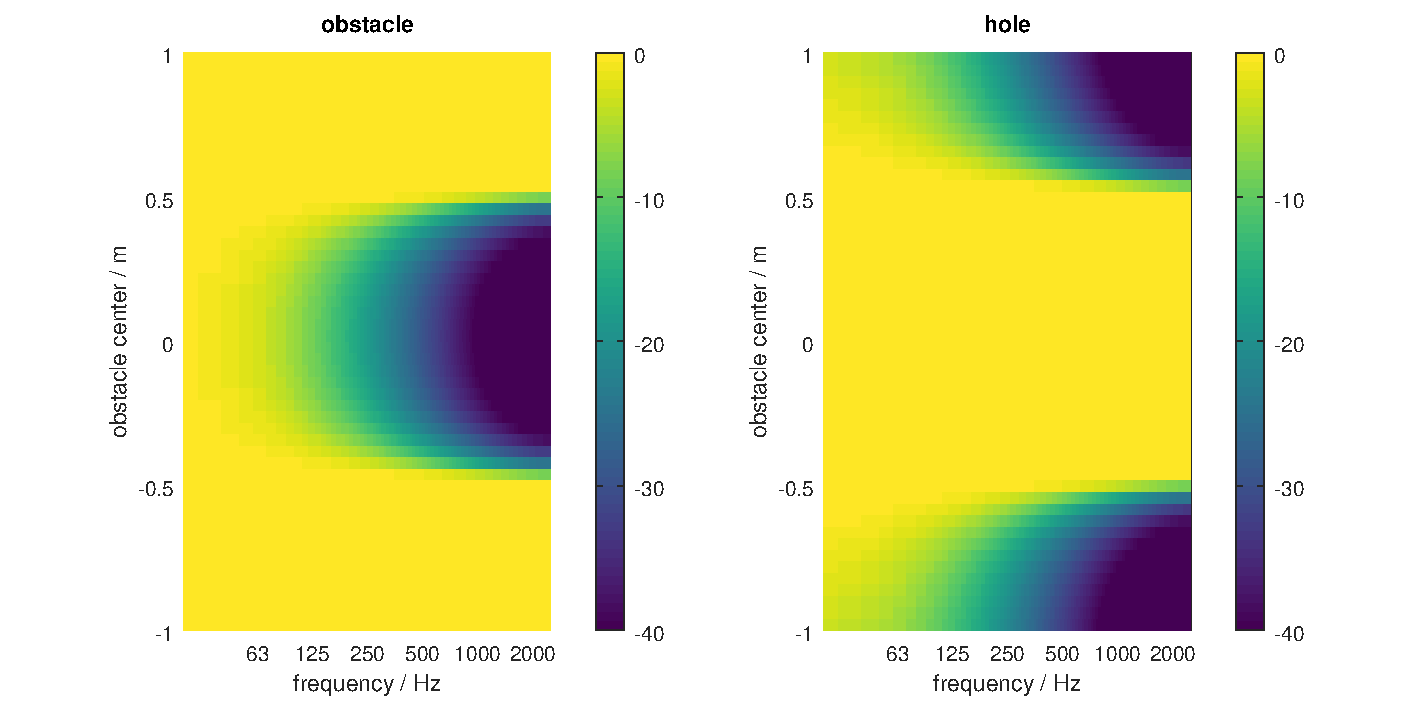
\includegraphics[width=\textwidth]{obstacle.pdf}}
    \caption{Frequency attenuation of a limited obstacle (left) and a hole (right) of 1 square meter, as a function of obstacle distance.}
    \label{fig:obstacle}
\end{figure}


\subsection{Masks: {\tt <mask ../>} element}\index{mask}\label{sec:mask}

Global masks affect the attenuation in a receiver, based on the receiver position.
See Figure \ref{fig:masks}.

\begin{figure}[htb]
    \centering
    \fbox{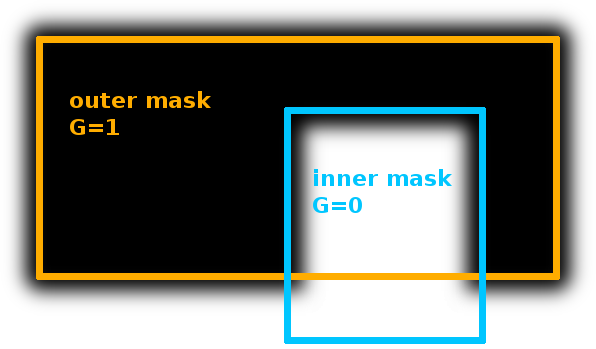
\includegraphics[width=\textwidth]{masks.png}}
    \caption{Global masks example.}
    \label{fig:masks}
\end{figure}

%\begin{figure}[ht]
%\centerline{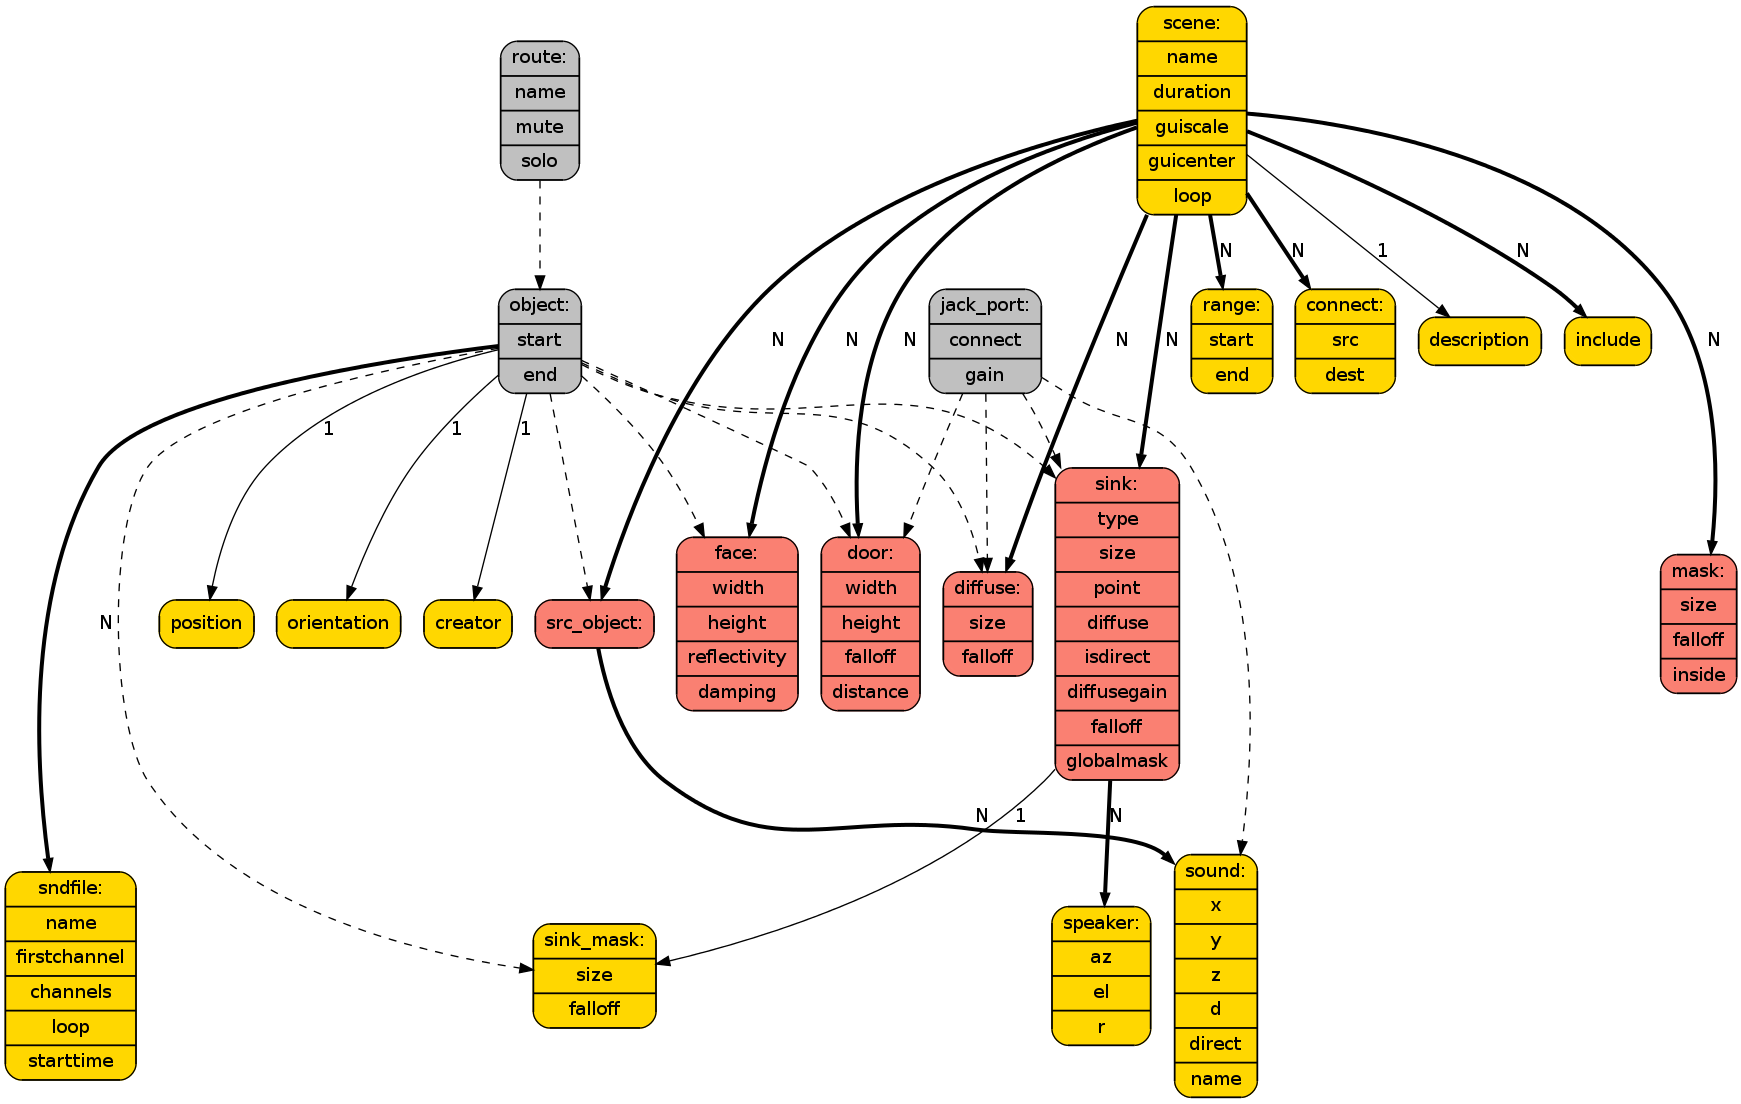
\includegraphics[width=\columnwidth]{filestructure.png}}
%\caption{\label{fig:filestructure}{\it File structure and relations between nodes.}}
%\end{figure}

\clearpage

\section{General purpose modules}\label{sec:module}\index{modules}

External modules which do not directly interact with the acoustic
model of the virtual acoustic environment can be loaded as dynamic
libraries.
%
These modules may analyse or modify the session data, or simply
provide some additional functionality.
%
Modules can be added to a session file within the
\verb!modules!, e.g.,
\begin{lstlisting}[numbers=none]
  <modules>
    <simplecontroller actor="/*/out" ... />
  </modules>
\end{lstlisting}

\input{secmodules.tex}

\section{Actor modules}\label{sec:actormod}

Actor modules can be used in the same way as general purpose modules,
however, their purpose is to change or query the position one or more
objects by using an actor name definition:
\begin{lstlisting}[numbers=none]
<simplecontroller actor="/scene/obj" .../>
\end{lstlisting}
Name matching with \verb!*! is possible. For example, we can choose all the objects from the scene, whose names start with \verb!N!:

\attr{actor="/scene/N*"}

Or if we have more than one scenes, we can choose all the objects called \verb!out! from all scenes:

\attr{actor="/*/out"}

\input{secactmodules.tex}

\clearpage

\section{Audio plugins}\index{Audio plugins}

Each sound vertex \elem{sound}, each diffuse sound field
\elem{diffuse}, and each receiver \elem{receiver} can contain a list
of audio plugins for processing and analysis, such as tone generators
or speech analysis for lip synchronization modeling.
%
These audio plugins are specified within the \elem{plugins} section
within a \elem{sound} or \elem{receiver} element, e.g.:
\tscexample[linerange={9-14},firstnumber=9]{example_audioplugins}
%\begin{lstlisting}[numbers=none]
%<source name="car">
%  <sound name="wheel" z="-0.5">
%    <plugins>
%      <sndfile name="wheelsound.wav" levelmode="rms" level="85"/>
%      <sine f="1000" a="70"/>
%    </plugins>
%  </sound>
%</source>
%\end{lstlisting}

Audio plugins may share their variables via OSC.
%
See the list of OSC variables to check which variables can be
accessed.

Audio plugins are processed in the order they appear in the
configuration within the \elem{plugins} section. For sound vertices,
they are processed before the sound is handed to the acoustic
model. For receivers, audio plugins are processed after the post
processing function of the render format.

\input{secapmodules.tex}

\clearpage

\section{Adding diffuse reverberation}\label{sec:reverb}

\tascar{} is not capable of rendering physically or perceptually
correct diffuse or late reverberation.
%
However, it is still possible to add diffuse reverberation by means of
external tools, e.g., feedback delay networks (FDN) or convolution
tools.
%
To add diffuse reverberation, a room microphone needs to be added to
the scene, configured to volumetric mode (see section
\ref{sec:volumetric}, page \pageref{sec:volumetric}), and configured
to exclude diffuse sources from rendering (attribute
\attr{diffuse="false"}), see also example file \verb!example_diffreverb.tsc!:
%
\tscexamplepriv[linerange={40-42},firstnumber=40]{example_diffreverb}
%
The output of the reverberation tool needs to be in B-format,
Furse-Malham normalization and ACN channel order (wyzx). This output is
handled in \tascar{} the same way as any other diffuse sound field
(see Section \ref{sec:diffuse} on page \pageref{sec:diffuse}):
%
\tscexamplepriv[linerange={34-36},firstnumber=34]{example_diffreverb}
%
The appropriate reverberation tool can be started using the
\elem{system} module, and connections can be made using \elem{connect}
elements at the end of the session file:
%
\tscexamplepriv[linerange={44-50},firstnumber=44]{example_diffreverb}
%
The gain may need to be adjusted according to \citet{Grimm2015c}.
%
It is recommended to validate the resulting outcome both, perceptually
and by measuring the resulting impulse responses.
%
The GNU Octave/MATLAB tools provided with \tascar{} should be
sufficient in most cases (e.g., \verb!t60.m!, \verb!iacc.m!,
\verb!plot_t30.m!, \verb!tascar_ir_measure.m!).

A new method of adding reverb is described in \ref{sec:reverbelem}.

\section{Calibration and level metering}\index{calibration}\index{level}

\tascar{} offers a level meter for each primary or diffuse sound
field and receiver. In the level meters, root-mean-square (RMS)
values in dB SPL, averaged over the past two seconds, are shown.  In
\tascar{}, internal values are measured in Pa. This means that a
sinusoid with an amplitude of one corresponds to a level of 91 dB
SPL. The level of sound sources corresponds to the anechoic free field
level in a distance of 1~m.

Each input port (\refelem{sound} element) and output port
(\refelem{receiver} element) of \tascar{} can be calibrated with the
calibration level attribute \indattr{caliblevel}.

At the input, a full-scale sine wave corresponds to
\attr{caliblevel}$-3$~dB (because the RMS of a sine wave is $-3$ dB).
%
This means that in case of the sine wave, the level of that sound
source is 91 dB SPL, in a 1~m distance and anechoic conditions.
%
The last bit is important: In virtual acoustics we cannot easily
calibrate the level of sound sources at the listening position.
%
In anechoic conditions this can be calculated with the $\frac1r$
amplitude law, but in case of reflections this $\frac1r$ law is not
valid anymore.

For the sine wave the CREST-factor (difference between peak and RMS
level) is 3 dB, but for speech this is roughly 20-24 dB.
%
Thus typically for speech one will need a much higher \attr{caliblevel} than
93~dB, because otherwise a full-scale speech signal would result in
only 70 dB SPL.
%
Typically, any speech test software will have some output calibration value.
%
In case of the Oldenburg Measurement Applications (OMA) this is the
same as the \attr{caliblevel} of \tascar{}.
%
Most likely the value of it will be in the order of 120 dB SPL
(similar to the \attr{caliblevel} of the \tascar{} receiver).
%
If the \attr{caliblevel}-value of the speech test software is known, exactly
the same value should be used for the \tascar{} input \attr{caliblevel}.
%
In that case, the input level meters of \tascar{} should show the same
values as the output level meters of the speech test.

For a calibration of speaker layouts, it is recommended to use the
tool ``tascar\_spkcalib''.

To measure the sound pressure level in a virtual acoustic environment,
one can place an omni-directional microphone at the position of the main
output receiver.
%
This omni-directional level meter should show the same numbers as a
real physical sound level meter in the center of the physical
reproduction system.
%
The sound level meters need to be configured to ``unweighted'',
``Z-weighted'' or ``C-weighted'' settings.
%
Please be aware of the fact that in ``unweighted'' mode the background
noise levels can be in the order of 40-60 dB, due to ventilation of
the room, door slamming in the building, steps, nearby trains and
plains etc., which contain extremely low frequencies.

\index{frequency weighting}\index{level meter}
The \tascar{} level meters support three different frequency
weightings: ``Z'' or unweighted mode, ``C'' weighting (62.5~Hz to
4~kHz) and a ``bandpass'' weighting (500~Hz to 4~kHz).

\subsection{Calibrating speaker layouts with {\tt tascar\_spkcalib}}

All loudspeaker-based rendering methods (e.g., those depending on a
loudspeaker layout file) should result in identical levels at the
listening positions for virtual sound sources from the directions of
the speakers (the levels of interpolated virtual sources may differ
due to differences in the rendering method).
%
The broadband calibration of loudspeaker layouts consists of three
steps: a) calibrate gain differences between loudspeakers b) calibrate
the reference level for point source rendering, and c) calibrate the
gain correction for diffuse sound field rendering.
%
The tool \verb!tascar_splcalib! can be used to perform these steps.

The levels are calibrated using the ``nsp'' rendering method. When
using ``hoa2d'' or ``neukom\_basic'' receiver types, the level
differences were tested to be below 0.25~dB. When using ``vbap'' or
``wfs'', the level differences are tested to be below 2.5~dB.

\begin{figure}[htb]
    \centering
    \fbox{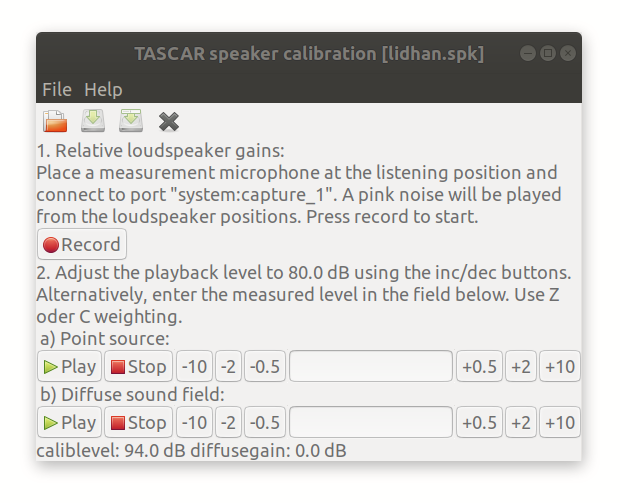
\includegraphics[width=0.7\textwidth]{tascarspkcalib.png}}
    \caption{Loudspeaker calibration window.}
    \label{fig:spkcalib}
\end{figure}

To (re-)calibrate a loudspeaker layout file, open it with
\verb!tascar_splcalib!, e.g., by double-clicking it in the file
explorer.
%
The application has four control areas (see Fig.\ \ref{fig:spkcalib}):
the menu and toolbar at the top of the application window can be used
to open, save and close loudspeaker layout files.
%
Below is the area for measurement of gain differences between
loudspeakers, followed by an area for measurement of the reference
level for point source rendering.
%
At the bottom of the window the area for calibration of the diffuse
rendering gain can be found.

The microphone signal can be also used for level metering, if calibrated correctly.
%
The calibration value can be configured via the global configuration
variable \verb!tascar.spkcalib.miccalib! (see Section
\ref{sec:globalconfig}).
%
Please make sure to properly calibrate before using it, and after any
changes in the chain from microphone to AD converter.

\subsubsection{Calibrating a loudspeaker array for the first time}

The default calibration level in TASCAR is 94~dB SPL. The default test
tone level is 80~dB SPL. If the actual calibration level is far above
the default value, then pressing the ``play'' button will result in
excessive sound levels. Therefore it is recommended to decrease the
sound level by pressing the ``-10 dB'' button several times. Then
press ``play'', and increase the level using the ``+10 dB'', ``+2 dB''
and ``+0.5 dB'' buttons until the level reaches approximately
80~dB. Then press the stop button. From here, follow the instructions
for a re-calibration.

\subsubsection{Re-calibration of a loudspeaker array}

For re-calibration of a loudspeaker array, you will need a measurement
microphone (omni-directional characteristics, flat frequency response
from 60 to 4000 Hz), and a sound level meter with Z or C
weighting. The calibration test tone is a pink noise in the frequency
range from 62~Hz to 4~kHz. Connect the microphone to the port
\verb!system:capture_1! (or change the setting
\verb!tascar.spkcalib.inputport! to the jack port name of your
microphone, see Section \ref{sec:globalconfig} for details), and place
it at the listening position. Now press ``Record'' to start a
recording of levels. The sound will be played from the directions of
the loudspeakers. After the recording is completed, the mean recording
level and its range are displayed next to the ``Record'' button. If
the recording level is very low (below -50 dB), then verify the
connection and configuration of your microphone. Also the level range
should not exceed 20 dB, otherwise inspect the connections of the
loudspeakers.

In the next step, play the test tone as a point source using the
``play'' button in the point source section. Enter the sound pressure
level measured at the listening position into the level entry field in
the window, or use the decrement and increment buttons to adjust the
playback level. When finished with this step, press the ``Stop''
button.

Now, repeat the same procedure, but with a diffuse test sound, by
pressing the ``Play'' button in the diffuse calibration area. Enter
the level reading in the appropriate field, or adjust the level using
the increment/decrement buttons.

If all steps are completed, press the ``Save'' or ``Save as'' button
at the top of the window. The changes are stored into the loudspeaker
file. It is recommended to review the calibration and gain values
using an editor.


\clearpage

\section{Interfacing from MATLAB and GNU/Octave}

For the interface between \tascar{} and MATLAB or GNU/Octave a set of
scripts are provided in \verb!/usr/share/tascar/matlab!.
%
There are the following scripts available:

\subsection{\tt tascar\_ctl}

This function can be used for some basic actions. For details see
function help in MATLAB/GNU Octave.

\begin{itemize}
\item Loading a scene, which already exists:\\
  \verb!h = tascar_ctl('load','filename.tsc')!
\item Controlling the transport:\\
  \verb!tascar_ctl( 'transport', h, 'play' )!\\
  \verb!tascar_ctl( 'transport', h, 'locate', 15 )!
\item Closing a scene: \\
  \verb!tascar_ctl('kill',h )!
\item Creating a basic scene:\\
  \verb!tascar_ctl('createscene','filename','my_scene.tsc')!
\item Create an audio player:\\
  \verb!h = tascar_ctl('audioplayercreate',{sig1,sig2});!
  \verb!tascar_ctl('audioplayerselect',1);!\\
  \verb!tascar_ctl('audioplayerselect',2);!\\
  \verb!tascar_ctl('kill',h )!
\end{itemize}

%         'load', 'kill', 'createscene', 'transport', 'audioplayercreate'

An example of the usage of this (and other MATLAB/GNU Octave functions) can be
found in \verb!example_controlTASCAR.m!.

\subsection{\tt generate\_scene}

In \tascar{}, virtual acoustic environments are defined in an xml file
format.
%
User can write such a file on his own or create it using MATLAB/GNU Octave
function \verb!generate_scene!.
%
This function can generate a simple scene with one speaker based
receiver, N sources distributed on a circle around the receiver and K
virtual loudspeakers, also equally distributed on a circle around the
receiver.
%
There are a couple of parameters which can be specified by a user -
the file name, the number of sources and loudspeakers, radius of the
circle, receiver type, as well as the length of a delay line.



\subsection{\tt tascar\_jackio}

When we already have an XML file with a virtual environment, we may
want to start performing some measurements using MATLAB/GNU Octave.
%
The function \verb!tascar_jackio! is used to play and record sound via
jack (jack audio connection kit).
%
It means that we are playing the sound using ports responsible for the
sources in the virtual scene and recording the sound using ports
responsible for the receiver in the scene.
%
Usually, it will be a test signal (for example white noise) played
back and recorded (for example to compute the impulse response of the
virtual environment).

At the input of the function, we have to specify input and output jack
ports which will be used for playing and recording the signal:
\begin{lstlisting}[numbers=none]
[y,fs,bufsize] = tascar_jackio( x, ...
                                'output', csOutputPorts, ...
                                'input', csInputPorts );
\end{lstlisting}
Here \verb!output! is a list of port connections to which the sound
vector \verb!x! will be sent (typically corresponding to the virtual
sound sources in a \tascar{} scene, e.g.,
\verb!{'render.scene:src.0'}!).
%
The number of channels in \verb!x! must match the number of output
port connections.
%
Accordingly, \verb!input! is a list of input port connections from
which the content of \verb!y! will be read (e.g., the receiver outputs
of a scene, or audio hardware inputs).
%
If you specify writable clients as \verb!input!, e.g., the sound card
outputs, then \verb!tascar_jackio! will connect to all readable input
ports which are connected to the specified writable port.
%
This can be used to record the signal sent to the loudspeakers, even
if it is a mixture from several scenes.
%
The number of channels in \verb!y! will be the number of elements in
the input variable.

For more information, type \verb!help tascar_jackio! (usage
information), or \verb!tascar_jackio help! (full list of parameters).

\subsection{\tt tascar\_ir\_measure}

Measure an impulse response using a sine sweep method after \cite{Farina2000}.

\subsection{\tt send\_osc}\label{sec:sendosc}

The properties of objects placed in the scene or for example the
transport state can be manipulated from outside \tascar{} using
OSC-messages.
%
The parameters (properties) of an object which can be changed by
sending an OSC message to \tascar{} are called "OSC variables".
%
For example, in MATLAB/GNU Octave it can be done by using the provided
function \verb!send_osc! (for UDP transport) or \verb!send_osc_tcp!
(for TCP transport).

The functions \verb!send_osc!  and \verb!send_osc_tcp! are functions
by which we can control a \tascar{} session and objects in a \tascar{} scene.
%
The default OSC port is 9877, listening on all network devices.
%
For more control, we can use the attributes
\attr{srv\_addr} and \attr{srv\_port} to the element \elem{session}, e.g.,
\begin{lstlisting}[numbers=none]
<session srv_addr="" srv_port="9999">
\end{lstlisting}
To check the list of variables and the OSC server port in a \tascar{}
session, select the sub-menu ``OSC variables'' in the menu ``view''
from the main menu bar.
%
Each OSC variable has its path and type.
%
On the right side of each variable path, you can see also its type in
brackets.
%
\verb!(f)! means a floating point number, \verb!(fff)! means a vector
with 3 floating point numbers (it can for example correspond to 3
coordinates for the position), \verb!(i)! means integer etc.

Function \verb!send_osc! requires specifying the destination host
(e.g., 'localhost') and port number, the path, and the variable
values, e.g.,
\begin{lstlisting}[numbers=none]
send_osc( 'localhost', 9877, '/scene_name/object_name/pos', ...
          pos_x, pos_y, pos_z, euler_z, euler_y, euler_x );
\end{lstlisting}
%
where \verb!pos_x!, \verb!pos_y!, \verb!pos_z! are the cartesian
coordinates in meters and \verb!euler_z!, \verb!euler_y!,
\verb!euler_x! are the rotations around $x$, $y$, and $z$-axis in
degrees.
%
They are always relative to the position and orientation specified in
the scene definition file.

Position can also be specified using only 3 numbers:

\begin{lstlisting}[numbers=none]
send_osc('localhost',9877,'/scene_name/object_name/pos',...
         pos_x,pos_y,pos_z)!
\end{lstlisting}
Orientation of the object can be also changed using:
\begin{lstlisting}[numbers=none]
send_osc('localhost',9877,'/scene_name/object_name/zyxeuler',...
         euler_z euler_y,euler_x)
\end{lstlisting}
To mute or solo one object, we use:
\begin{lstlisting}[numbers=none]
send_osc('localhost',9877,'/scene_name/object_name/solo',1)
send_osc('localhost',9877,'/scene_name/object_name/mute',1)
\end{lstlisting}

Sending OSC messages can also be used for starting, stoping or placing a scene at the arbitrary point in time:

Stop/start a scene:
\begin{lstlisting}[numbers=none]
send_osc('localhost',9877,'/transport/stop')
send_osc('loclhost',9877,'/transport/start')
\end{lstlisting}
Go back to beginning / 4th second:
\begin{lstlisting}[numbers=none]
send_osc('localhost',9877,'/transport/locate',0)
send_osc('localhost',9877,'/transport/locate',4)
\end{lstlisting}


\clearpage

\section{Command line interfaces}

All command line applications of \tascar{} start with the prefix
\verb!tascar_!. To get a list of valid command line options, use the
flag \verb!-h! or \verb!--help!.

\begin{itemize}
\item \verb!tascar_cli!\\
  Load \tascar sessions from command line (no GUI support)
\item \verb!tascar_renderfile!\\
  This command line tool can be used for rendering the image source model of a single scene in a
  \tascar{} session with audio input from a sound file and saving the rendered signal to a sound file.
  Common usage example:
  \begin{lstlisting}[numbers=none]
  tascar_renderfile -i input_file.wav -o output_file.wav tascar_scene.tsc
  \end{lstlisting}

  The size of the input file \verb!input_file.wav! (number of audio
  channels) has to correspond with the number of sources in the
  scene. The size of the file \verb!output_file.wav!, which will be
  created after calling this tool, will correspond to the number of
  output channels of the receiver used in the scene. In case of
  multi-channel output (e.g., speaker based receiver types), the order
  follows the order of the channel definition in the \tascar{}
  files. This may differ from the order of jack ports, because some
  jack front ends sort ports alphabetically.

  Other options:

  \begin{lstlisting}[numbers=none]
  -h
  --help

  -s #
  --scene=#

  -i #
  --inputfile=#

  -o #
  --outputfile=#

  -t #
  --starttime=#

  -d
  --dynamic

  -f #
  --fragsize=#

  -0 #
  --ismmin=#

  -1 #
  --ismmax=#

  -v
  --verbose
  \end{lstlisting}
\item \verb!tascar_renderir!\\
This command line tool is used for rendering the impulse response of a \tascar{} scene. Common usage example:
  \begin{lstlisting}[numbers=none]
  tascar_renderir -o output_file.wav -f 44100 -1 2 tascar_scene.tsc
  \end{lstlisting}
The impulse response will be stored in \verb!output_file.wav!. \verb!44100! is the sampling rate and \verb!2! is the highest rendered image source order.

\item \verb!tascar_lslsl!\\
This command line tool outputs a list of available Lab Streaming Layer (LSL) streams.
\item \verb!tascar_lsljacktime! \\
  Create an LSL stream with jack time
\item \verb!tascar_hdspmixer! \\
  Interface to HDSP9652
\item \verb!tascar_jackio! \\
  Play and record wav files via jack.
\end{itemize}


\clearpage

\section*{List of symbols and definitions}\label{sec:symbols}

\begin{tabular}{ccl}
symbol                    & dimension   & variable                                                                                                    \\
\hline
$t$                       & scalar      & sampled time                                                                                                \\
$N$                       & scalar      & number of receiver output channels                                                                          \\
$K$                       & scalar      & number of point sources in a scene                                                                          \\
$L$                       & scalar      & number of diffuse sound fields in a scene                                                                        \\
$\mathbf{p}_{src}$        & $1\times 3$ & source position                                                                                             \\
$\mathbf{p}_{rec}$        & $1\times 3$ & receiver position                                                                                           \\
$\mathbf{p}_{spk}$        & $1\times 3$ & loudspeaker position in receiver coordinate system                                                          \\
$(\varrho,\varphi,\theta)$ & $1\times 3$ & Spherical coordinates, distance $\varrho$, azimuth $\varphi$, elevation $\theta$\\
$\mathbf{D}$, $d$         & $N\times 4$ & first order Ambisonics decoder matrix                                                                       \\
$\mathbf{w}$, $w_n$       & $1\times N$ & driving weights for point source at relative position $\mathbf{p}_{rel}$                                    \\
$\mathbf{z}(t)$, $z_n(t)$ & $1\times N$ & receiver output signal                                                                                      \\
$y_k(t)$                  & scalar      & acoustic model output signal for $k$-th point source                                                        \\
$\mathbf{f}_l(t)$         & $1\times 4$ & first order Ambisonics signal for $l$-th diffuse sound field                                                     \\
$\mathbf{O}_{rec}$        & $3\times 3$ & receiver orientation matrix                                                                                 \\
$\mathbf{p}_{rel}$        & $1\times 3$ & relative source direction $\mathbf{p}_{rel}= \mathbf{O}_{rec}^{-1} (\mathbf{p}_{src} - \mathbf{p}_{rec})^T$ \\
$r=||\mathbf{p}_{rel}||$  & scalar      & distance between source and receiver                                                                        \\
\end{tabular}

The receiver orientation is defined by
\begin{eqnarray}
\mathbf{O}_{rec}       & =              & \mathbf{O}_x \left(\mathbf{O}_y \mathbf{O}_z\right) \label{eq:orientation}\\
\mathbf{O}_x           & =              &
\left(
\begin{array}{ccc}
1                      & 0              & 0                                                   \\
0                      & \cos(\Omega_x) & -\sin(\Omega_x)                                     \\
0                      & \sin(\Omega_x) & \cos(\Omega_x)                                      \\
\end{array}
\right)
                                                                                              \\
\mathbf{O}_y           & =              &
\left(
\begin{array}{ccc}
\cos(\Omega_y)         & 0              & -\sin(\Omega_y)                                     \\
0                      & 1              & 0                                                   \\
\sin(\Omega_y)         & 0              & \cos(\Omega_y)                                      \\
\end{array}
\right)                                                                                       \\
\mathbf{O}_z           & =              &
\left(
\begin{array}{ccc}
\cos(\Omega_y)         & -\sin(\Omega_y & 0                                                   \\
\sin(\Omega_y)         & \cos(\Omega_y) & 0                                                   \\
0                      & 0              & 1                                                   \\
\end{array}
\right)                                                                                       \\
\hat{\mathbf{O}}_{rec} & =              & \left(
\begin{array}{cc}
1                      & 0                                                                    \\
0                      & \mathbf{O}_{rec}^{-1}
\end{array}\right)\label{eq:foarot}
\end{eqnarray}

\clearpage

\section{Appendix}

\bibliography{tascar}

\lstlistoflistings

\begin{table}[htb]
\begin{tabular}{llll}
Type                      & $N$       & panning                                     & diffuse decoding                                                                             \\
\hline
{\tt omni}                & 1         & $w_n=1$                                     & $d_{1,1} = 1$                                                                                \\
{\tt vmic}                & 1         & $w_n=1+a(\tilde p_{rel,x}-1)$                                     & $d_{1,1} = \sqrt{2}(1-a)$, $d_{1,2} = a$                                                                               \\
{\tt cardioid}            & 1         & $w_n=\frac12 \left(\cos(\varphi) + 1\right)$ & $d_{1,1} = 1$                                                                               \\
{\tt ortf} & 2 & ORTF microphone & $\max r_E$\\
{\tt amb\_3h0v}           & 7         & $w_n=\left\{
\begin{array}{cl}
\sqrt{2}                  & n=1                                                                                                                                                    \\
\cos(\frac{n}{2}\varphi)   & n\, \textrm{even}                                                                                                                                     \\
\sin(\frac{n-1}{2}\varphi) & n\, \textrm{odd}
\end{array}\right.$       & $d_{n,n}=1,\, n=\{1,2,3\}$                                                                                                                             \\
{\tt amb\_3h3v}           & 16        &
$w=
\left(\begin{array}{c}
w_w                                                                                                                                                                                \\w_y\\w_x\\w_z\\w_v\\w_t\\w_r\\w_s\\w_u\\w_q\\w_o\\w_m\\w_k\\w_l\\w_n\\w_p
\end{array}
\right)=
\left(\begin{array}{c}\sqrt{2}                                                                                                                                                     \\
\cos(\theta)\sin(\varphi)                                                                                                                                                          \\ %y
\cos(\theta)\cos(\varphi)                                                                                                                                                          \\ %x
\sin(\theta)                                                                                                                                                                       \\ %z
2 w_x w_y                                                                                                                                                                          \\ %v
2 w_z w_y                                                                                                                                                                          \\ %t
\frac12 (3 w_z^2 - 1)                                                                                                                                                              \\ %r
2 w_z w_x                                                                                                                                                                          \\ %s
w_x^2 - w_y^2                                                                                                                                                                      \\ %u
(3 w_x^2 - w_y^2) w_y                                                                                                                                                              \\%q
2.598076 w_z w_v                                                                                                                                                                   \\ %o
0.726184 (5 w_z^2 - 1) w_y                                                                                                                                                         \\ %m
\frac12 w_z (5 w_z^2 - 3)                                                                                                                                                          \\ %k
0.726184 (5 w_z^2 - 1) w_x                                                                                                                                                         \\ %l
2.598076 w_z w_u                                                                                                                                                                   \\ %n
(w_x^2 - 3 w_y^2) w_x                                                                                                                                                              \\ %p
\end{array}\right)$   & $d_{n,n}=1,\, n=\{1,2,3,4\}$                                                                                                                               \\
{\tt neukom\_basic}   & user def. & $w_n=1+2\sum_{l=1}^{order}\cos(l\varphi_n)$                                                                                                    \\
{\tt neukom\_inphase} & user def. & $w_n=\cos(0.5\varphi_n)^{order}$                                                                                                               \\
{\tt hoa2d}           & user def. & see \cite{Daniel2001} for details.                                                                                                             \\
{\tt nsp}             & user def. & $w_{\argmin\left\{\norm[\big]{\frac{\mathbf{p}_{rel}}{\norm{\mathbf{p}_{rel}}} - \frac{\mathbf{p}_{spk}}{\norm{\mathbf{p}_{spk}}}}\right\}}=1$ \\
{\tt hann}            & user def. & $w_n = \left(\frac12 + \frac12 \cos\left(\min\left\{\left|\frac{N}{2} \varphi_n\right|,\pi\right\}\right)\right)^\gamma$                       \\
{\tt vbap}, {\tt vbap3d}            & user def. & see \cite{Pulkki1997} for details.                                                                                                             \\
%{\tt vbap3d}         & user def. & $ w_n=?$ & $d=?$                                                                                                                               \\
\end{tabular}
\caption{Specification of receiver types. $d_{n,wxyz}=0$ except for
  the given entries. $(\varrho,\varphi,\theta)$ is the source position
  in spherical coodinates in the receiver coordinate
  system. $\varphi_n$ is the azimuthal angular distance between
  loudspeaker $n$ and the sound source.}\label{tab:receivers}
\end{table}

\begin{figure}[p]
  \includegraphics[width=\columnwidth]{acousticmodel.pdf}
  \caption{Signal flow in the acoustic model.}\label{fig:acmodel}
\end{figure}

\printindex

\newpage
\TASCARcopyright{}

\end{document}

% Local Variables:
% ispell-local-dictionary: "en_US"
% End:

%%  LocalWords:  TASCAR Ambisonics binaural reflectivity facegroup
%%  LocalWords:  anechoic sinusoid SPL RMS directivity cardioid LSL
%%  LocalWords:  jackd POSIX tascar MATLAB matlab OSC UDP TCP
%%  LocalWords:  bandpass
